%!TEX TS-program = pdflatex
% dissertation.tex -- main dissertation file
%
% Wisconsin dissertation template
% Copyright (c) 2008-2009 William C. Benton.  All rights reserved.
%
% This program can redistributed and/or modified under the terms
% of the LaTeX Project Public License Distributed from CTAN
% archives in directory macros/latex/base/lppl.txt; either
% version 1 of the License, or (at your option) any later version.
%
% This program includes other software that is licensed under the
% terms of the LPPL and the Perl Artistic License; see README for details.
%
% You, the user, still hold the copyright to any document you produce
% with this software (like your dissertation).
%

%%% You'll want ``oneside'' for the deposit version, but probably not for any versions that don't need to meet the UW requirements
\documentclass[12pt,oneside,letterpaper,oldfontcommands]{memoir}
\usepackage[margin=1.2in]{geometry}


\usepackage{amssymb}
\usepackage{wrapfig}
\usepackage{amsmath}
\usepackage{caption}
\usepackage{subcaption}
\usepackage{xcolor}
\usepackage{multirow}
\usepackage{paralist}
\usepackage{url}
\usepackage{hyperref}
\hypersetup{
	colorlinks = true,
	urlcolor = {green}, urlbordercolor = {green},
	citecolor = {blue},
	linkbordercolor = {green}
}
%\usepackage{my_base}
\usepackage{amsmath}
\usepackage{amssymb}
\usepackage{amsthm}
\usepackage{mathtools}
\usepackage{amsmath,amsfonts,amssymb,amsthm,color,hyperref,amscd}
\usepackage{times,paralist}

\newcommand{\omitme}[1]{}

% preamble.tex -- packages to include
%
% Wisconsin dissertation template
% Copyright (c) 2008 William C. Benton.  All rights reserved.
%
% This program can redistributed and/or modified under the terms
% of the LaTeX Project Public License Distributed from CTAN
% archives in directory macros/latex/base/lppl.txt; either
% version 1 of the License, or (at your option) any later version.
%
% This program includes other software that is licensed under the
% terms of the LPPL and the Perl Artistic License; see README for details.
%
% You, the user, still hold the copyright to any document you produce
% with this software (like your dissertation).

%% You should use natbib
\IfFileExists{natbib.sty}{%
\usepackage{natbib}%
}{}

%% You probably need appendix, if you want appendices
\IfFileExists{appendix.sty}{%
\usepackage{appendix}%
}{}

%% the spacing in memoir is weird, you'll need to use this
\DisemulatePackage{setspace}
\usepackage[onehalfspacing]{setspace}

%% List setup; the ``hanglist`` environment will allow you to have
%% nicely-typeset enumerated lists (i.e. with the numbers hanging in
%% the margins).  You need at least version 2.1 of enumitem.sty.  If
%% you don't have enumitem installed at all, hanglist will just be an
%% alias for enumerate.

%%%%% commented by zihang
\IfFileExists{enumitem.sty}{%
\usepackage[inline]{enumitem}%
}
%\IfFileExists{enumitem.sty}{%
%\usepackage[loadonly]{enumitem}[2007/06/30]%
%\newlist{hanglist}{enumerate}{1}% 
%\setlist[hanglist]{label=\arabic*.}%
%\setlist[hanglist,1]{leftmargin=0pt}%
%}{%
%\newenvironment{hanglist}{\begin{enumerate}}{\end{enumerate}}%
%}
%%%%%%%%%%%%%%%%%%%%%%%%%%%%%%%%

%% Comment out any of these that you don't want
\usepackage{amssymb}
\usepackage{amsmath}
\usepackage{amsthm}
%\usepackage{theorem}
\usepackage{hyperref}

\IfFileExists{mathpartir.sty}{%
\usepackage{mathpartir}%
}{}

%%%%% LISTINGS package and setup
\IfFileExists{listings.sty}{%
\usepackage{listings}%
}{}



%% Get rid of ugly borders around PDF hyperlinks (e.g. for cross-references, bib entries, or URLs)
\hypersetup{pdfborder = 0 0 0}

%% You want microtype.
\IfFileExists{microtype.sty}{%
\usepackage[protrusion=true,expansion=true]{microtype}%
}{}

%\pagestyle{thesisdraft}

% Surround parts of graphics with box
\usepackage{boxedminipage}

%% booktabs (thx to Nate Rosenblum for bringing this beautiful package
%% to my attention)
\IfFileExists{booktabs.sty}{%
\usepackage{booktabs}%
}{}

% This is now the recommended way for checking for PDFLaTeX:
\usepackage{ifpdf}

%% Avoid ugly "Type 3" fonts
\usepackage{lmodern}
\usepackage[LY1]{fontenc}

%% Substitute your favorite serif and sans fonts here....
\IfFileExists{tgpagella.sty}{%
% TeX Gyre pagella, like Palatino
\usepackage{tgpagella}%
}{}

\usepackage[LY1]{eulervm}

\ifpdf
\usepackage[pdftex]{graphicx}
\else
\usepackage{graphicx}
\fi

\usepackage{makeidx}
\makeindex

{\theoremstyle{plain}
\newtheorem{thm}{Theorem}[chapter]
\newtheorem{cor}[thm]{Corollary}
\newtheorem{define}[thm]{Definition}
\newtheorem{exmpl}[thm]{Example}
}
{\theoremstyle{remark}
\newtheorem{rmk}[thm]{Remark}
}

\newtheoremstyle{customsty1}
{3pt}%
{3pt}%
{}% --- body font
{}% --- indent amount
{\bfseries}% --- Theorem head font
{:}% --- Punctuation after head
{.5em}% --- space after head
{}% --- theorem head spec (can be left empty, meaning 'normal')

% Define 'newtheorems' that use ``customsty1''
{\theoremstyle{customsty1} 
}


%%% NB: the ``deposit'' chapter- and page- styles should conform to UW
%%% requirements.  If you are producing a pretty version of your
%%% dissertation for web use later, you will certainly want to make
%%% your own chapter and page styles.

\makechapterstyle{deposit}{%
  \renewcommand{\chapterheadstart}{}
  \renewcommand{\printchaptername}{}
  \renewcommand{\chapternamenum}{}
  \renewcommand{\printchapternum}{\parbox{2em}{\MakeLowercase{\Large\scshape\thechapter{}}} }
  \renewcommand{\afterchapternum}{}
  \renewcommand{\printchaptertitle}[1]{%
  \raggedright\Large\scshape\MakeLowercase{##1}}
  \renewcommand{\afterchaptertitle}{%
  \vskip\onelineskip \hrule\vskip\onelineskip}
}

\makepagestyle{deposit}
 
\makeatletter
 
\renewcommand{\chaptermark}[1]{\markboth{#1}{}}
\renewcommand{\sectionmark}[1]{\markboth{#1}{}}
 
\makeevenfoot{deposit}{}{}{}
\makeoddfoot{deposit}{}{}{}
\makeevenhead{deposit}{\thepage}{}{}
\makeoddhead{deposit}{}{}{\thepage}
\makeatother

%%% set up page numbering for chapter pages to satisfy UW requirements
%%% NB: You will want to delete until the ``SNIP'' mark if you are
%%% making a ``nice'' copy
\copypagestyle{chapter}{plain}
\makeoddfoot{chapter}{}{}{}
\makeevenhead{chapter}{\thepage}{}{}
\makeoddhead{chapter}{}{}{\thepage}
%%% SNIP

%%% bib nonsense
\makeatletter
\newenvironment{wb-bib}[1]{%
  \chapter*{references}
\ifnobibintoc\else 
\phantomsection 
\addcontentsline{toc}{chapter}{References} 
\fi 
\prebibhook
  \begin{bibitemlist}{#1}}{\end{bibitemlist}\postbibhook}

\AtBeginDocument{%
  \@ifpackageloaded{natbib}{% natbib is loaded
    \addtodef{\endthebibliography}{}{\vskip-\lastskip\postbibhook}
    \@ifpackagewith{natbib}{sectionbib}{% with sectionbib option
      \renewcommand{\bibsection}{\@memb@bsec}}%
      {\renewcommand{\bibsection}{\@memb@bchap}}}%
  {}
  \@ifpackagewith{chapterbib}{sectionbib}{%
    \renewcommand{\sectionbib}[2]{}
    \renewcommand{\bibsection}{\@memb@bsec}}{}
}
\makeatother

% defs.tex -- wbepi environment for chapter epigraphs and other useful defs.
%
% Wisconsin dissertation template
% Copyright (c) 2008 William C. Benton.  All rights reserved.
%
% This program can redistributed and/or modified under the terms
% of the LaTeX Project Public License Distributed from CTAN
% archives in directory macros/latex/base/lppl.txt; either
% version 1 of the License, or (at your option) any later version.
%
% This program includes other software that is licensed under the
% terms of the LPPL and the Perl Artistic License; see README for details.
%
% You, the user, still hold the copyright to any document you produce
% with this software (like your dissertation).


%% put lstnewenvironment declarations here, if you're using listings

%% end lstnewenvironment declarations

%% I put convenience definitions that will go in several chapters here

%%%%% begin convenience definitions
\makeatletter
\newcommand{\wb@episource}{}
\newenvironment{wbepi}[1]{\begin{quote}\renewcommand{\wb@episource}{#1}\itshape}{\par\upshape \raggedleft --- \textsc{\wb@episource}\\ \end{quote}}
\makeatother

%%%%% SVN
\IfFileExists{svn-multi.sty}{%
\usepackage{svn-multi}%
%%% Uncomment the second one and comment out the first one if you want
%%% to include subversion revision information in each file.
\newcommand{\vcinfo}{}%
%\newcommand{\vcinfo}{\begin{centering}\fbox{\fbox{\parbox{5in}{Author: \svnauthor\\Revision: \svnfilerev\\Last changed on: \svnfiledate\\URL: \svnkw{HeadURL}}}}\\[1em]\end{centering}}%
}{%
\newcommand{\svnidlong}[4]{}%
\newcommand{\svnfilerev}{}%
\newcommand{\svnauthor}{}%
\newcommand{\svnfiledate}{}%
\newcommand{\svnkw}{}%
\newcommand{\vcinfo}{}%
}
\usepackage{hyperref}

% put bunch of \newcommand below

%%%%% end convenience definitions
 %all packages and definitions can go here
\usepackage[framemethod=TikZ]{mdframed}

% \newtheorem{theorem}{Theorem}
% \newtheorem{lemma}{Lemma}
% \newtheorem{proposition}{Proposition}
% \newtheorem{definition}{Definition}
% \newtheorem{corollary}{Corollary}
% \newtheorem{remark}{Remark}
% \newtheorem{assumption}{Assumption}

\def\EE{\mathbb{E}}
\def\II{\mathbb{I}}
\def\PP{\mathbb{P}}
\def\RR{\mathbb{R}}


\def\cA{\mathcal{A}}
\def\cC{\mathcal{C}}
\def\cD{\mathcal{D}}
\def\cH{\mathcal{H}}
\def\cI{\mathcal{I}}
\def\cL{\mathcal{L}}
\def\cM{\mathcal{M}}
\def\cP{\mathcal{P}}
\def\cS{\mathcal{S}}
\def\cT{\mathcal{T}}
\def\cU{\mathcal{U}}
\def\cW{\mathcal{W}}
\def\cX{\mathcal{X}}
\def\cY{\mathcal{Y}}
\def\cZ{\mathcal{Z}}

\newcommand{\SPD}{\text{SPD}}
\newcommand{\VAR}{\text{VAR}}
\newcommand{\EXP}{\text{Exp}}
\newcommand{\LOG}{\text{Log}}

\mdfdefinestyle{MyFrame}{%
    linecolor=blue!50!white,
    outerlinewidth=1pt,
    roundcorner=5pt,
    innertopmargin=0.5\baselineskip,
    innerbottommargin=0.5\baselineskip,
    innerrightmargin=10pt,
    innerleftmargin=10pt,
    backgroundcolor=blue!10!white}
% thesisdefs.tex

% This is mostly adapted from withesis.cls.  The original copyright
% notice for withesis.cls follows, preceded by two percent signs (%%):

%% withesis.cls
%% LaTeX Style file for the University of Wisconsin-Madison Thesis Format
%% Adapted from the Purdue University Thesis Format
%% Originally by Dave Kraynie
%% Edits by Darrell McCauley
%% Adapted to UW-Madison format by Eric Benedict  (Noted with <EB>)
%% Updated to LaTeX2e by Eric Benedict 24 July 00
%% 
%%=============================================================================
%% Licensed under the Perl Artistic License.
%% see: http://www.ctan.org/tex-archive/help/Catalogue/licenses.artistic.html
%% for more info...
%%=============================================================================

% withesis.cls is available from CTAN.  The modifications to this file
% are also licensed under the Perl Artistic License.

% --wb, 2008

\makeatletter

\newcounter {tocpage}
\newcounter {lofpage}
\newcounter {lotpage}
\newcounter {listofheading}

\newcommand\@thesistitlemedskip{0.2in}
\newcommand\@thesistitlebigskip{0.6in}
\newcommand{\degree}[1]{\gdef\@degree{#1}}
\newcommand{\project}{\gdef\@doctype{A masters project report}}
\newcommand{\prelim}{\gdef\@doctype{A preliminary report}}
\newcommand{\thesis}{\gdef\@doctype{A thesis}}
\newcommand{\dissertation}{\gdef\@doctype{A dissertation}}
\newcommand{\department}[1]{\gdef\@department{(#1)}}

\newenvironment{titlepage}
 {\@restonecolfalse\if@twocolumn\@restonecoltrue\onecolumn
  \else \newpage \fi \thispagestyle{empty}
% \c@page\z@ -- deleted: count title page in thesis
}{\if@restonecol\twocolumn \else \newpage \fi}

\gdef\@degree{Doctor of Philosophy}    %Default is PhD
%\gdef\@doctype{A dissertation}         %Default is dissertation
\gdef\@doctype{A preliminary report}


\gdef\@department{(Computer Sciences)} % Default is Electical Engineering
\gdef\@defensedate{10/18/2021 {\color{red}-- in includes/thesisdefs.tex}}% Default is a long time from now.
\gdef\@committee{ \color{red}
  Name FamilyName1, Assistant Professor, Department\\ 
  Name FamilyName2, Professor, Department\\  
  Name FamilyName3, Assistant Professor, Department\\
  Vikas Singh (Advisor), Professor, Biostatistics and Medical Informatics
  }

\renewcommand{\maketitle}{%
  \begin{titlepage}
%-----------------------------------------------------------------------------
% -- The thesis office doesn't like thanks on title page.  Put it in
% -- the acknowledgments.  This is here so you don't have to change
% -- your titlepage when converting from report style. -> from Purdue, but I
%        left it here since it seems compatible with UW-Madison, Eric
%-----------------------------------------------------------------------------
    \def\thanks##1{\typeout{Warning: `thanks' deleted from thesis titlepage.}}
    \let\footnotesize\small \let\footnoterule\relax \setcounter{page}{1}
    \begin{center}
      {\textbf{\expandafter\expandafter{\@title}}} \\[\@thesistitlebigskip]
       by \\[\@thesistitlemedskip]
      \@author \\[\@thesistitlebigskip]
      \@doctype\ submitted in partial fulfillment of \\
      the requirements for the degree of\\[\@thesistitlebigskip]
      \@degree \\[\@thesistitlemedskip]
      \@department \\[\@thesistitlebigskip]
      at the \\[\@thesistitlemedskip]
      UNIVERSITY OF WISCONSIN--MADISON\\[\@thesistitlemedskip]
      \@date
    \end{center}
%    \hspace*{-0.7in}Date of final oral examination: \@defensedate \\[\@thesistitlemedskip]
    \hspace*{-0.4in}Date of preliminary examination: \@defensedate \\[\@thesistitlemedskip]
%    \hspace*{-0.7in}The dissertation is approved by the following members of the 
    \hspace*{-0.4in}The examination is approved by the following members of the 
    Oral Committee:\\
    \@committee
  \end{titlepage}
  \setcounter{footnote}{0}
  \setcounter{page}{1} %title page is NOT counted
  \let\thanks\relax
  \let\maketitle\relax \let\degree\relax \let\project\relax \let\prelim\relax
  \let\department\relax
  \gdef\@thanks{}\gdef\@degree{}\gdef\@doctype{}
  \gdef\@department{}
  %\gdef\@author{}\gdef\@title{}
}


%=============================================================================
% ABSTRACT
%=============================================================================
% The abstract should begin with two single-spaced lines describing
% the author and title in a standard format.  After these lines comes
% the standard abstract.
%=============================================================================
\def\abstract{
  \chapter*{Abstract}
  \addcontentsline{toc}{chapter}{Abstract}
  \relax\markboth{Abstract}{Abstract}}
\def\endabstract{\par\newpage}


%=============================================================================
% UMI ABSTRACT
%=============================================================================
% The UMI abstract should begin with the author and title in a standard format.
% After the author comes the advisor and university. After these lines comes
% a bunch of double spaced text to make up the standard abstract.
% After the abstract, the advisor's approval signature follows.
% This page is not numbered and is delivered seperately to the thesis office.
%=============================================================================

\def\advisortitle#1{\gdef\@advisortitle{#1}}
\def\advisorname#1{\gdef\@advisorname{#1}}
\gdef\@advisortitle{Professor}
\gdef\@advisorname{Cheer E.\ Place}

\def\umiabstract{
             \thispagestyle{empty}
                  \addtocounter{page}{-1}
                \begin{center}
                  {\textbf{\expandafter\uppercase\expandafter{\@title}}}\\
                  \vspace{12pt}
                  \@author \\
                  \vspace{12pt}
                  Under the supervision of \@advisortitle\ \@advisorname\\
                  At the University of Wisconsin-Madison
                \end{center}
}

\def\endumiabstract{\vfill \hfill\@advisorname\par\newpage}


%============================================================================
% VERBATIMFILE
%============================================================================
% \verbatimfile{<filename>}    for verbatim inclusion of a file
% - Note that the precise layout of line breaks in this file is important!
% - added the \singlespace - EB
%============================================================================
\def\verbatimfile#1{\begingroup \singlespace
                    \@verbatim \frenchspacing \@vobeyspaces
                    \input#1 \endgroup
}


%=============================================================================
% SEPARATOR Pages
%   Creates a blank page with a text centered horizontally and vertically.
%   The page is neither counted nor numbered.
%   These pages are required in the thesis format before sections such
%   as appendices, vita, bibliography, etc.
%=============================================================================
\def\separatorpage#1{
  \newpage
  \thispagestyle{empty}
  \addtocounter{page}{-1}
  \null
  \vfil\vfil
  \begin{center}
    {\textbf{#1}}
  \end{center}
  \vfil\vfil
  \newpage}


%=============================================================================
% COPYRIGHTPAGE
%=============================================================================
% The copyright must do the following:
% - start a new page with no number
% - place the copyright text centered at the bottom.
%=============================================================================
\def\copyrightpage{
  \newpage
  \thispagestyle{empty}    % No page number
  \addtocounter{page}{-1}
  \chapter*{}            % Required for \vfill to work
  \begin{center}
   \vfill
   \copyright\ Copyright by \@author\ \@date\\
   All Rights Reserved
  \end{center}}


%=============================================================================
% GLOSSARY
%=============================================================================
% The glossary environment must do the following:
% - produce the table of contents entry for the glossary
% - start a new page with GLOSSARY centered two inches from the top
%=============================================================================
\def\glossary{
  \chapter*{GLOSSARY}
  \addcontentsline{toc}{chapter}{Glossary}}
\def\endglossary{\par\newpage}

%=============================================================================
% NOMENCLATURE
%=============================================================================
% The nomenclature environment must do the following:
% - produce the table of contents entry for the nomenclature section
% - start a new page with NOMENCLATURE centered two inches from the top
%=============================================================================
\def\nomenclature{\separatorpage{DISCARD THIS PAGE}
  \chapter*{Nomenclature}
  \addcontentsline{toc}{chapter}{NOMENCLATURE}}
\def\endnomenclature{\par\newpage}

%=============================================================================
% CONVENTIONS
%=============================================================================
% The conventions environment must do the following:
% - produce the table of contents entry for the nomenclature section
% - start a new page with CONVENTIONS centered two inches from the top
%=============================================================================
\def\conventions{\separatorpage{DISCARD THIS PAGE}
  \chapter*{Conventions}
  \addcontentsline{toc}{chapter}{CONVENTIONS}}
\def\endconventions{\par\newpage}


%=============================================================================
% COLOPHON
%=============================================================================
% The colophon environment must do the following:
% - produce the table of contents entry for the nomenclature section
% - start a new page with COLOPHON centered two inches from the top
%=============================================================================
%\def\colophon{\separatorpage{DISCARD THIS PAGE}
%  \chapter*{Colophon}
%  \addcontentsline{toc}{chapter}{Colophon}}
%\def\endcolophon{\par\newpage}

%=============================================================================
% LIST OF SYMBOLS
%=============================================================================
% The list of symbols environment must do the following:
% - produce the table of contents entry for the list of symbols section
% - start a new page with LIST OF SYMBOLS centered two inches from the top
%=============================================================================
\def\listofsymbols{\separatorpage{DISCARD THIS PAGE}
  \eject
  \chapter*{LIST OF SYMBOLS}
  \addcontentsline{toc}{chapter}{LIST OF SYMBOLS}}
\def\endlistofsymbols{\par\newpage}

%=============================================================================
% VITA
%=============================================================================
% The vita environment must do the following:
% - produce a separator page with the word vita centered
% - produce the table of contents entry for the vita
% - start a new page with VITA centered two inches from the top
%=============================================================================
\def\vita{
%  \separatorpage{VITA}         % UW doesn't require this EB
  \chapter*{VITA}
  \addcontentsline{toc}{chapter}{VITA}}
\def\endvita{\par\newpage}

%=============================================================================
% ACKNOWLEDGMENTS
%=============================================================================
% The acknowledgments environment must do the following:
% - start a new page with ACKNOWLEDGMENTS centered two inches from the top
%=============================================================================
\def\acks{
  \chapter*{Acknowledgments}
}
\def\endacks{\par\newpage}

%=============================================================================
% DEDICATION
%=============================================================================
% The dedication environment must do the following:
% - start a new page
% - center the text vertically
% - include the text in a center environment
%=============================================================================
\def\dedication{
  \newpage
  \null\vfil
  \begin{center}}
\def\enddedication{\end{center}\par\vfil\newpage}

%=============================================================================
% DATE
%=============================================================================
%\def\today{\ifcase\month\or
  %January\or February\or March\or April\or May\or June\or
  %July\or August\or September\or October\or November\or December\fi
  %\space\number\day, \number\year}
\newcount\@testday
\def\today{\@testday=\day
  \ifnum\@testday>30 \advance\@testday by -30
  \else\ifnum\@testday>20 \advance\@testday by -20
  \fi\fi
  \number\day\ \
  \ifcase\month\or
    January \or February \or March \or April \or May \or June \or
    July \or August \or September \or October \or November \or December
    \fi\ \number\year
}


%  Single counter for theorems and theorem-like environments:
\newtheorem{theorem}{Theorem}[chapter]
\newtheorem{assertion}[theorem]{Assertion}
\newtheorem{claim}[theorem]{Claim}
\newtheorem{conjecture}[theorem]{Conjecture}
\newtheorem{corollary}[theorem]{Corollary}
\newtheorem{definition}[theorem]{Definition}
\newtheorem{example}[theorem]{Example}
\newtheorem{figger}[theorem]{Figure}
\newtheorem{lemma}[theorem]{Lemma}
\newtheorem{prop}[theorem]{Proposition}
\newtheorem{remark}[theorem]{Remark}

%=============================================================================
% TABLE OF CONTENTS; LIST OF FIGURES; LIST OF TABLES
%=============================================================================
% In report style, \tableofcontents, \listoffigures, etc. are always
% set in single-column style.  @restonecol is used to keep track of
% whether we need to switch back to double column style after the toc.
%
% The only known problem now is that the first page with the new
% layout is too long.  The problem seems to be that the change to
% textheight doesn't take place on the first page.  Even if it's the
% first line in the table of contents macro.  Presumably the same
% problem also occurs in the lof and lot.
%
% I'm taking a shot at fixing the problem by dropping in a throw-away
% page between the change to the height parameters and the start of
% the chapter.  Isn't elegance wonderful?
%
%=============================================================================

% \def\@tableof#1#2#3#4#5{
% { % limit scope of following declarations!!
%   \@restonecolfalse\if@twocolumn\@restonecoltrue\onecolumn\fi
%   \addtolength{\textheight}{-40pt}       % -24-16
%   \addtolength{\majorheadskip}{-40pt}    % -24-16
%   \addtolength{\headheight}{52pt}        %  36+16
%   \addtolength{\headsep}{-12pt}          % -12
%   \separatorpage{DISCARD THIS PAGE}
%   \chapter*{#1}
%   #5
%   \relax\markboth{#1}{#1}
%   \hbox to \hsize{#2 \hfil Page}
%   \singlespace
%   \setcounter{#3}{0}
%   \setcounter{listofheading}{1}  % change from 0 to 1 by mccauley, 14may93
%   \def\@oddhead{\vbox to \headheight{\vspace{4pt}
%     \hbox to \hsize{\hfil\textrm{\thepage}} \vfil
%     \ifnum\value{#3}=1
%       \ifnum\value{listofheading}=2
%         \hbox to \hsize{Appendix\hfil} \vspace{4pt} \fi
%       \ifnum\value{listofheading}=1
%         \stepcounter{listofheading} \fi
%       \hbox to \hsize{#2 \hfil Page}
%     \else
%       \setcounter{#3}{1}
%     \fi}}
%   \def\@evenhead{\vbox to \headheight{\vspace{4pt}
%     \hbox to \hsize{\textrm{\thepage}\hfil} \vfil
%     \ifnum\value{#3}=1
%       \ifnum\value{listofheading}=2
%         \hbox to \hsize{Appendix\hfil} \vspace{4pt} \fi
%       \ifnum\value{listofheading}=1
%         \stepcounter{listofheading} \fi
%       \hbox to \hsize{#2 \hfil Page}
%     \else
%       \setcounter{#3}{1}
%     \fi}}
%   \@starttoc{#4}  \if@restonecol\twocolumn\fi
%   \newpage
% }}
% 
% \def\tableofcontents{\@tableof{TABLE OF CONTENTS}{}{tocpage}{toc}{}}
% 
% \def\listoffigures{
%   \@tableof{LIST OF FIGURES}{Figure}{lofpage}{lof}
%   {\protect\addcontentsline{toc}{chapter}{LIST OF FIGURES}}}
% 
% \def\listoftables{
%   \@tableof{LIST OF TABLES}{Table}{lotpage}{lot}
%   {\protect\addcontentsline{toc}{chapter}{LIST OF TABLES}}}

%=============================================================================
% BIBLIOGRAPHY
%=============================================================================
% The thebibliography environment executes the following commands:
%
%  o start a new 'chapter' with BIBLIOGRAPHY as the heading
%  o produce a separator page for the bibliography
%
%  \def\newblock{\hskip .11em plus .33em minus -.07em} --
%      Defines the `closed' format, where the blocks (major units of
%      information) of an entry run together.
%
%  \sloppy  -- Used because it's rather hard to do line breaks in
%      bibliographies,
%
%  \sfcode`\.=1000\relax --
%      Causes a `.' (period) not to produce an end-of-sentence space.
%=============================================================================
% \altbibtitle
%   The default title for the References chapter is ``LIST OF REFERENCES''
%   Since some people prefer ``BIBLIOGRAPHY'', the command
%   \altbibtitle has been added to change the chapter title.
%   This command does nothing more than change REFERENCES to BIBLIOGRAPHY
%============================================================================
\def\@bibchaptitle{Bibliography}
\def\altbibtitle{\def\@bibchaptitle{Bibliography}}
\def\thebibliography#1{
  %\separatorpage{\@bibchaptitle}
  \global\@bibpresenttrue
  \chapter*{\@bibchaptitle\markboth{\@bibchaptitle}{\@bibchaptitle}}
  \addcontentsline{toc}{chapter}{\@bibchaptitle}
  \vspace{0.375in}    % added to match 4 line requirement
  \interlinepenalty=10000 % added to prevent breaking of bib entries
  \singlespace\list
  {[\arabic{enumi}]}{\settowidth\labelwidth{[#1]}\leftmargin\labelwidth
    \advance\leftmargin\labelsep \usecounter{enumi}}
  \def\newblock{\hskip .11em plus .33em minus -.07em}
  \sloppy
  \sfcode`\.=1000\relax}
\let\endthebibliography=\endlist



\makeatother


%\svnidlong{$LastChangedBy$}{$LastChangedRevision$}{$LastChangedDate$}{$HeadURL: http://freevariable.com/dissertation/branches/diss-template/dissertation.tex $} 


\let\ab\allowbreak
%%%%%%%%%%%%%%%%%%%%%%%%%%%%%%%%%%%%%%%%%%%%%%%%%%%%%%

% \title{Identifying Problem-Specific Subsets of Features and Samples in Modern Learning via Geometry and Independence}
% \title{Low-Dimensional Subspace Identification and Analysis in Modern Learning via Geometry and Independence}
\title{Identifying Feature, Parameter, and Sample Subsets in Modern Learning and Imaging Analysis}
\author{Ronak Mehta}
\department{Computer Sciences Department}
\date{2022}

\begin{document}

%%% Uncomment the following if your .bib contains references that you will not  explicitly cite, but that should be in the final bibliography:
% \nocite{*}

\maketitle
\tableofcontents
\newpage

% 
% the space of the data $X \in \cX$

% subset of input space $\cS \subseteq \cX$, $S \subseteq X$

% model space $\theta \in \Theta$

% subset of the model space $\cP \subseteq \Theta$, $P \subseteq \theta$

-------------------------

\begin{verbatim}
todos:
    intro
        expand
        yunyang/zihang
        more related work for each specific selection
    background
        diff geom
        graphs, conditional indep
        hyp test
        tensors
        unlearning
    add full paper texts
    smoothing/transition
    abstract
    conclusions/future/open
    acks
\end{verbatim}


% Include each chapter.tex file
\chapter{Introduction} \label{chap:intro} 

Modern applications of machine learning have become ubiquitous, 
to the point where almost all
interactions with so-called ``smart"
technologies involve some
call and response with some form of
learned predictor.
The large scale of these models,
up to billions of parameters in neural networks
allows for what would otherwise
be an unconstrained, infeasible learning task
to be possible via a highly parameterized model.
These parameterizations have enabled 
human-level performance on learning tasks
previously thought to have been insurmountable
for any potential artificial intelligence system.
The high accuracy and generalization of these large scale models notwithstanding,
a number of parallel questions have arisen with respect to 
the performance of these models.
What features are most important for prediction?
Which samples were most important for my training?
Can we understand when a model is certain or uncertain about its output?
Are there layers in my network that have learned a particular subtask?
Questions of robustness, bias, influence, fairness, and importance have become central questions to contemporary machine learning research.

Classical machine learning and statistics have found new life in these subfields: traditional learning methods 
have been studied with these questions in mind for many decades.
Linear regressors, decision trees, and support vector machines
have all been analyzed under these lenses,
and as the modern machine learning community
has returned to these questions
so has a renewed interest in their methods of analysis.
Research interest focuses
particularly on the differences
associated with moving from classical under-parametrized models to
modern \textbf{over-parameterized} models: where
the model dimension vastly outnumbers the number
of input samples, and may even be comparable to 
the \textit{entire sample space.}
While nascent, these approaches 
attempt to fill the gap between
statistical and deep models to enable similar measures of sample influence, feature importance, and model analysis. 

% Significant progress in the modern development of machine learning has
% been built upon connections and patterns identified across myriad
% interdisciplinary fields of study.
% Up through the mid 2000's, 
% many of these methods were inspired by and interested in 
% highly focused and constrained problems. 
% With a reasonably sized input domain, could a model of roughly equal size be used to
% predict some output?
% Linear regressors, decision trees, and support vector machines were all answers to these questions, with their own
% varying degrees of scaling and complexity.
% These methods necessitated carefully constructed formulations with specific restrictions to the learnable function class,
% enabling straightforward analysis 
% for provable performance guarantees 
% and easy identification of critical training samples and important input features.

% Contemporary machine learning, however, has a vastly different modus operandi. 
% Driven in large part by the exponential growth of available computation via Moore's Law, \textit{deep learning} has fallen squarely in the realm of \textbf{over-parameterized} models.
% With these overparametrizations and computation capacity, the typical learning questions posed as maximizing accuracy or reducing error have largely been addressed for even large scale problems.
% As such, complementary questions have led to subfields focusing on other performance measures, such as robustness, fairness, interpretability, and explainability.
% Many solutions to these questions end up looking back at answers found for the under- or non-parametrized settings.
% While nascent, these approaches 
% attempt to fill the gap between
% statistical and deep models to enable similar measures of sample influence, feature importance, and model analysis. 
% Most notable amongst these newer approaches is that of (Self)-Attention in Neural Networks \citep{sutskever2014sequence,vaswani2017attention}.
% Other proposals 
% end up looking back at the types of analysis typical of those more classical under-parametrized or nonparametrized methods.

% Not limited to previous developments in learning or computation theory, the arguably most valuable contributions toward the exponential reduction in model error can be attributed to influences and intuitions taken
% from biology, psychology, neuroscience, and even XXX \citep{srivastava, etc}.
% Perhaps one explanation as to why this phenomenon exists may be attributed to the way in which deep learning evolved. 
% The classical learning goal of function approximation lends itself nicely to a system which allows for arbitrary complexity via simple changes (e.g., addition of neural network layers). % Foundational works building on the original neural networks particularly have taken advantage of constraining this space of functions to search over: 
% the most seminal case being those of convolutional filters for imaging data. 
% While ``constraints" of this form have helped tremendously in model performance on modern vision and language machine learning tasks (GANs, Recurrent Networks, Residual Layers, Transformers, etc.), the ability to identify \textit{subsets} of important samples, input features, and model parameters has lagged significantly behind the development of these methods.
% Recently larger interest has been taken by the community to understand and interpret models with this view, only after extremely large and opaque models have become ubiquitous.
%This lag directly explains the more recent interest in developing methods for understanding and interpreting large scale machine learning models.


\paragraph{A full picture.} Consider a dataset $\{X\}_{i=1}^n$ of size $n$ where each data point in the set $X$ is considered drawn from some underlying distribution over the domain $X \sim \cX^d$, with domain dimensionality $d$. A model $f$ is fit using a parametrizations $\theta \in \Theta$, with $\Theta$ the space of possible parametrization with some intrinsic dimension $p$. From an analysis perspective, we might be interested in any one of (a) subsets of input features $\cC \subseteq \cX$ that are important for the downstream task, (b) associating model subsets $\cP \subseteq \Theta$ with specific inputs or groups of inputs, or (c) subsets of samples $S \subseteq \{X\}^n$ equally of interest. While all three of these problems are closely related, they require different approaches. 

\begin{mdframed}[style=MyFrame]
\em 
\textbf{This thesis} focuses its main efforts on identifying these important subsets of sample, feature, and model space for feature association, model size reduction, model unlearning, and, fairness. Specifically, taking advantage of both existing statistical and geometric methods, we develop new methods for localizing subsets in both hypothesis testing and in deep learning frameworks.
\end{mdframed}

% Features
Feature selection in the case of typical regression or classification
% Typical regression or classification 
takes some form of learning parameters $\theta$ that allow for $\hat{y} = f_\theta(x)$ to be close to the true outcome of interest $y$.
While forms of data $X := (x,y)$ may simply be continuous and real-valued, modern machine learning has greatly expanded formulations of the classical learning problem to include a wide variety of structured learning problems \citep{nowozin2011structured}. 
Structure learning and identification has taken a few different forms (object detection, segmentation, etc.),
but has remained somewhat removed from traditional
statistical settings.
Consider the case when a high-dimensional input is used to predict an output with a highly-parametrized model. 
Once learned, obvious questions arise: are there specific low-dimensional spaces in either the input or the model space that are most important or necessary for the global learning problem of interest? Are there specific subspaces associated with particular subproblems of the global problem?
The machine learning literature has come up with a number of ways to identify analogs of these spaces, including extensions of sensitivity analysis to deep learning \citep{yeung2010sensitivity,zhang2015sensitivity}, and constructing and identifying nonzero model subsets via particular model choices such as activations \citep{selvaraju2017grad} and regularizers.
Attention has stood out as a popular method,
given its ease of implementation and interpretation \citep{sutskever2014sequence,vaswani2017attention}.
By learning dimensions of a given input that are particularly important, either in a hard (binary) or soft (continuous weighting) manner, model builders are better able to understand and interpret what a model has learnt.

The specific ideas of attention notwithstanding, many of these existing methods are far removed from traditional hypothesis testing frameworks, and
there remains a gap in direct identification of subsets and structures in these spaces that can be defined in statistically rigorous manners.

\paragraph{A specific example.} Consider a traditional machine learning classification task in which we would like to predict whether an individual has a specific disease condition based on a medical resonance image (MRI) scan of their brain. Our input feature $x$ may consist of a 3D-array of values lying in $\RR^{x\times y\times z}$ measuring some intensity of the imaging modality at each voxel, indexed by a tuple $(i,j,k)$.
Our outcome variable $y$ may simply be a binary label of whether the input scan has been labeled by a radiologist as one demonstrating typical disease characteristics.
Using an off the shelf 3D convolutional neural network with adjustments to match our input size, we can very quickly set up and train a system to predict disease presence with a high degree of accuracy.

While attention can be directly applied to the network in order to identify ``hotspots" in the input space relating to the learned classification task, there is no guarantee that the regions identified are truly related to disease.
Given the high-dimensional nature of the input and the relatively small sample size associated with medical imaging data, it is very likely that an area of interest identified may be an intricacy of the training samples used rather than truly a region of disease signal.
Methods of generalization may help to increase confidence in identified regions, but statistical guarantees remain out of reach.

Furthermore, most recent problems associated with medical data have moved past simple difference detection: trends over time, and the ability to predict {\em future} development has by far become the setting of most interest.
Given an image of a healthy individual, is it possible to predict what their scan, or their future disease diagnosis, may be up to 10, 20, or more years in the future?
If a number of scans have been collected over some timeframe, can the \textit{trajectory} of the individuals' development be extrapolated to estimate progression?
As traditional models extended for temporal analysis grow in both size and complexity,
a number of subproblems explicitly related to model and input subspaces arise. Here we address two such problems: \textbf{statistically rigorous identification of temporally evolving subsets}, and \textbf{characterizations of deep models that enable efficient training of recurrent models with large scale time-varying data}.

With the rapid growth of AI and machine learning applications has come valid concerns regarding both guarantees of privacy.
Recent technology legislation has made the importance clear in all aspects of data use,
and particular projects and groups have demonstrated that machine learning is not independent of
this need \citep{Exposing}.
A new issue raised within this intersection is the ``right to be forgotten".
If a model has been trained with a particular users' data, 
they should have some recourse or right
to both remove their data from the training set,
and also know that the model has not learned from their data.
On the surface, this poses a significant problem for model builders
and organizations that spend large amounts
of time and resources in 
training deep learning models.
As we will see, 
\textbf{identification of model parameter subsets}
that are particularly important
for a particular sample's influence
in a model enables \textit{efficient machine unlearning}.

% para - connections to geometric deep learning, graph NNs, etc.


A sample's particular influence on model parameters aside, the identification of influential samples or subsets of samples more generally is of independent interest. 
Traditionally a rigorous area of study under classical statistics, outlier detection and accounting have become a subfocus for many within the machine learning community as well \citep{golatkar2020eternal,golatkar2020forgetting,huang2020feature,ren2019likelihood}.
While subgroups of input samples may be outliers, it is more often the case that they represent known heterogeneity within the data. 
These differences are typically marked using 
group information known a priori, and 
most learning tasks aim to learn tasks
in a \textit{subgroup-independent} manner.
Optimization and regularization methods with this focus come under the umbrella of model fairness, and instead of identifying and boosting independences within the model or data, we aim to minimize them.
However, many existing methods do not scale well as the number of subgroups grows, as is often the case when intersections of protected classes must be considered. In the sequel we identify and construct a particular solution for \textbf{groupwise fairness that enables efficient in the loop fairness regularization}.

\clearpage
\begin{mdframed}[style=MyFrame]
{\bf Thesis Goal: }
\em Identify, construct, and evaluate methods for subset identification in machine learning input, feature, and model spaces, taking advantage of inherent geometric and statistical structures that naturally arise in application domains. 
Application focus is put on the temporal evolution of medical imaging data, as observed through traditional biomarkers and longitudinal imaging modalities.
\end{mdframed}

\section{Thesis Scope and Contributions}

In this thesis we explore the intersections of classical statistical and geometric constructions with modern machine learning methods. 
Figure~\ref{fig:scope} shows the overall scope projected along three axes: feature, parameter, and sample spaces.
Below we briefly introduce the main problems studied in this thesis.
\begin{figure}[!ht]
    \centering
    % \includegraphics[width=0.99\linewidth]{scope.pdf}
    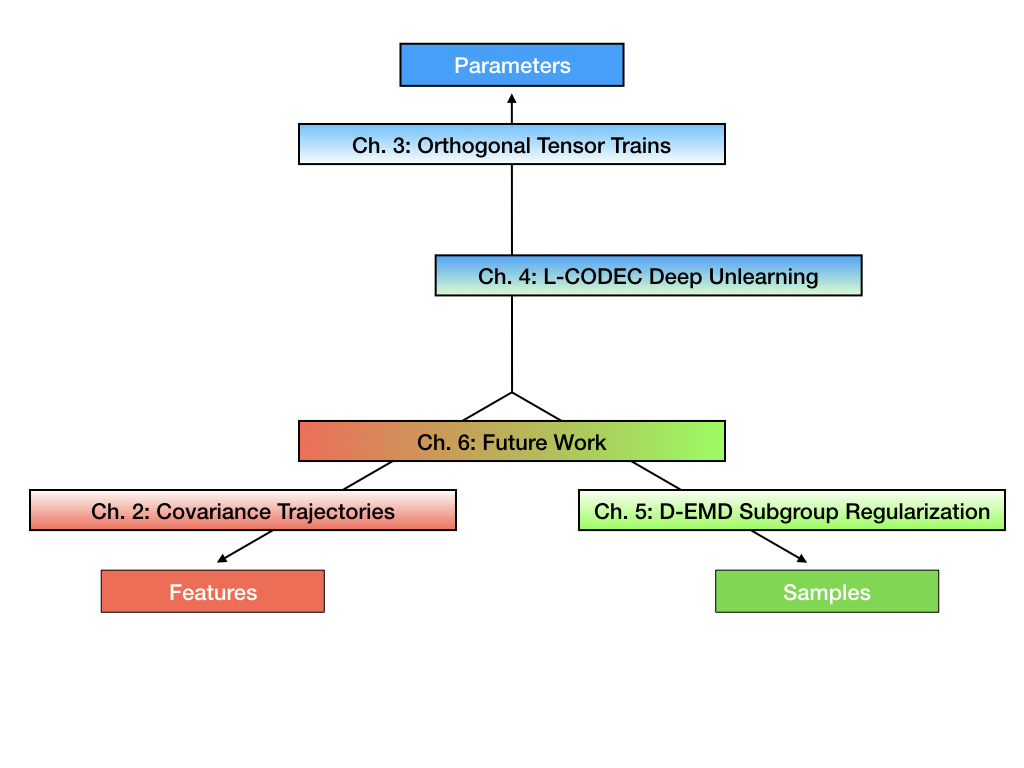
\includegraphics[width=0.95\linewidth]{_introduction/thesis_scope.png}
    \caption{Thesis scope, projected over three representative axes.}
    \label{fig:scope}
\end{figure}

\subsection{Second-Order Modeling and Group Difference Analysis over Time}

Recent results in coupled or temporal graphical models offer schemes for estimating the relationship structure 
between features when the data come from
related (but distinct) longitudinal sources. A novel application of these ideas is for analyzing group-level differences, i.e., in identifying if {\em trends} of estimated objects (e.g., 
covariance or precision matrices) are different across disparate conditions (e.g., gender or disease). Often, poor effect sizes make detecting the \textit{differential} signal 
over the {\em full} set of features difficult: for example, 
dependencies between only a {\em subset of features} may manifest differently across groups.
We first suggest
a parametric model 
for estimating trends in the space of $\SPD$ matrices as a function of one or more covariates.
We will then generalize scan statistics to graph structures, 
to search over distinct subsets of features (graph partitions) whose temporal dependency structure may show statistically 
significant group-wise differences.
We will theoretically analyze the Family Wise Error Rate (FWER) and bounds on Type 1 and Type 2 error. 
On a cohort of individuals with risk factors for Alzheimer's disease (but otherwise cognitively healthy), 
we aim to 
find scientifically interesting 
group differences where the default analysis, 
i.e., models estimated on the {\em full graph}, do not survive reasonable 
significance thresholds. 


\subsection{Efficient Tensor Representations for Feasible Temporal Deep Learning}

Modern deep networks have proven to be very effective for analyzing real world images.
However, their application in medical imaging is still in its early stages,
primarily due to the large dimension of three-dimensional images, requiring enormous convolutional or fully connected layers --
if we treat an image (and not image patches) as a sample. 
These issues only compound when the focus moves towards longitudinal analysis
through recurrent structures, and when a point estimate of model parameters is insufficient 
in scientific applications where a reliability measure is necessary.
Using insights from differential geometry, 
we will adapt 
the tensor train decomposition to construct networks
with significantly fewer parameters,
allowing us to train powerful recurrent networks on whole brain image volumes. 
We propose 
the \textit{orthogonal tensor train},
and demonstrate its ability to express a standard network layer both theoretically and empirically.
We will 
demonstrate its ability to 
effectively reconstruct whole brain volumes
with faster convergence and stronger confidence intervals
compared to the standard tensor train decomposition. 
We provide code and show experiments on the ADNI dataset
using image sequences to regress on a cognition related outcome.


\subsection{Practical Unlearning via Large-Scale Conditional Independence Testing}

%With AI systems extensively using personal %data for model training, 
Recent legislation has
led to interest in {\em machine unlearning}, i.e., removing specific training samples from a {\em predictive} model as if they never existed in the training dataset. 
Unlearning may also be required due to  corrupted/adversarial data or simply a user's updated privacy requirement.
For models which require no training ($k$-NN), 
simply deleting the closest original sample can be effective. 
%However, it is not clear how such approaches can be used to unlearn 
%models that contain rich information learned from the original data.
But this idea is inapplicable to models which learn richer 
representations.
%from data. 
%Recently, optimization-based unlearning estimators have been proposed, but 5their 
Recent ideas leveraging optimization-based updates
scale poorly with the model dimension $d$,  
due to 
inverting the Hessian of the loss function. %with an overall cost of $O(d^3)$ 
%is prohibitive.
We propose
a variant of a new conditional independence coefficient, 
L-CODEC, to identify a subset of the model parameters with the most semantic overlap on an individual sample level. 
Our approach completely avoids the need to invert a (possibly) huge matrix. 
By utilizing a Markov blanket selection, 
we premise
that L-CODEC is also suitable for deep unlearning,
as well as other applications in vision.
Compared to alternatives, L-CODEC makes approximate unlearning possible 
in settings that would otherwise be infeasible, 
including vision models used for face recognition, 
person re-identification 
and NLP models that may require unlearning samples identified for exclusion.


\subsection{Reducing Subgroup Fairness via High Dimensional Earth Mover's Distances}

Optimal transport has recently emerged as a useful tool for machine learning through its connections with geometry, statistical machine learning, and through practical algorithms. Existing methods that leverage optimal transport often  regularize using  a Wasserstein metric or by computing barycenters, for example. %which are effective when distributions are continuous and known, or when measures of interest are discrete.
% Our formulation allows for a discretization of continuous measures that drop in directly to classical  formulations of the Earth Mover's Distance. 
We will leverage optimal transport, except that we take advantage of a recently-introduced algorithm that computes a generalized earth mover's distance.
Not only is this algorithm computationally cheaper to compute compared to existing barycentric measures, but our method has the additional  advantage that gradients used for backpropagation can be directly read off of the forward pass computation, which leads to substantially faster model training.
We will provide technical details about this new regularization term and its properties, 
and 
experimental demonstrations of improved training speed over existing Wasserstein-style methods.

\subsection{Understanding Preclinical Alzheimer's Disease via Modern Technical Tools}

The final chapter of this thesis applies some of the tools developed above in analyzing preclinical Alzheimer's disease patients. 
In these studies, 
we aim to identify conditionally independent features and subjects that are particularly important to the prediction and estimation of
key disease outcomes,
as a function of a number 
of demographic, neuropsychological,
genetic,
and imaging data collected as 
part of an ongoing consortium 
to understand the progression
of Alzheimer's disease in younger, 
asymptomatic populations.

% This work is the most forward looking, and aims to be a stepping stone toward a rigorous 

\subsection{Outline}
In Chapters 2 through 5, we describe four perspectives to address subset identification.
Chapter 2 explores and focuses on the identification of feature subsets varying over time.
In Chapter 3 we describe a method of constraining the parameter space in a particular manner
that enables more efficient large scale neural networks.
Next, Chapter 4 provides a solution to the machine unlearning problem,
enabled through a particular conditional independence parameter selection scheme, vastly reducing network update costs.
Chapter 5 ends with a unique solution to subgroup fairness, 
where we take advantage of an efficient solution to
the $d$-dimensional earth mover's problem
to regularize large models when the number of subgroups can be large.
Chapter 6 describes future work, focused on applying a particular solution from Chapter 4 to understanding relationships among
disease indicators and biomarkers associated with developing Alzheimer's Disease.
\chapter{Localizing Group Differences over
Covariance Trajectories}\label{sec:covtraj}

Feature selection has become a core problem with the increase in dimensionality of learning problems.
Identifying and exploiting conditional independencies within data enables previously intractable problems to be solved,
and this chapter focuses on one particular angle along this direction.
% Multivariate data analysis exploiting the conditional independence structure between features or covariates using 
% undirected graphical models is now standard within any data analysis toolbox. 
When data are multivariate Gaussian, the zeros in the inverse covariance (precision) matrix give conditional independences 
among the variables \citep{lauritzen1996graphical}. 
Further, if the precision matrix is sparse, we can
derive dependencies between features when the data are high-dimensional and/or the number of measurements are small. 
The estimation of a graphical model
has been extensively studied
%in statistics and machine learning,
and a rich literature is available describing 
its statistical and algorithmic properties \citep{koller2009probabilistic,jordan1998learning}. 
For instance, the so-called \textit{graphical lasso} formulation uses an $\ell_1$-norm penalty on the 
precision matrix and is widely used, and consistency properties 
in the large $p$ regime \citep{cai2011constrained,friedman2008sparse,yuan2010high} are now well understood.
These formulations have also been extended to various transformations of Gaussian distributions (e.g., non-paranormal)
%, where the 
using rank statistics \citep{liu2009nonparanormal,xue2012regularized,liu2012high}.
%are a consistent estimator of 
%the precision matrix nonzero pattern 

{\em Coupled and Temporal Graphical Models.} 
%In various situations,
Often, data come from two (or more) disparate sources or multiple timepoints.
Within the last few years, a few proposals have 
described strategies for linking the sparsity patterns of multiple graphical models, e.g., using a fused lasso 
penalty \citep{danaher2014joint} \citep{yang2015fused}. Observe that 
%these ideas assume that the two (or more) models share a similar structure; 
if the data sources correspond to {\em longitudinal} acquisitions, we should expect 
the `structure' to gradually evolve.
%, which is discouraged in direct applications of the above idea. 
%in the case where the model is changing such a construction would not allow for identification of the evolving graph structure. 
% Several authors have offered generalizations to address this problem: \citep{zhou2010time} removes the assumption
% that each graph is independent and structurally `close'.
% Instead, \citep{zhou2010time} can be thought of as a growth model \citep{mcardle2000introduction} defined on these structures: they show how non-identically distributed graphs can be learned over time. 
% Recently, the nonparametric procedure in \citep{qiu2015joint} extends these ideas
% %via means
% to handle multiple sources, each with multiple samples.

The ideas in the literature so far to ``couple'' multiple graphical model estimation modules are mostly nonparametric \citep{zhou2010time, mcardle2000introduction,qiu2015joint}. 
While such a formulation offers benefits, in many estimation problems, 
parametric models may 
%require fewer samples (better convergence rates) and possibly, 
be more convenient for downstream statistical analysis,
particularly for hypothesis testing \citep{hardle1993comparing,geer2000empirical,roehrig1988conditions}.
% Given that the topic of \textit{coupled} graphical models, by itself, is fairly recent, algorithms for {\em parametric estimation} of 
% temporal or coupled Gaussian graphical models have not yet been heavily studied. 
\begin{figure*}[t]
  \centering
  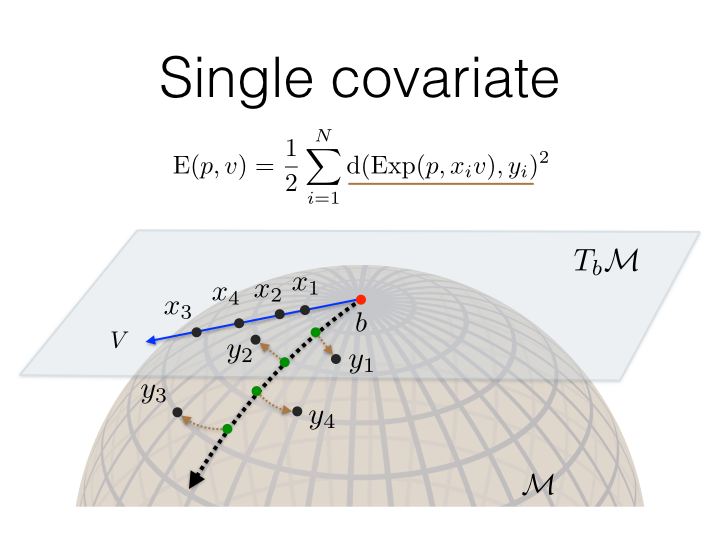
\includegraphics[width=0.49\textwidth,trim={10 40 10 220},clip]{chap2/MGLM1.png}
  %
    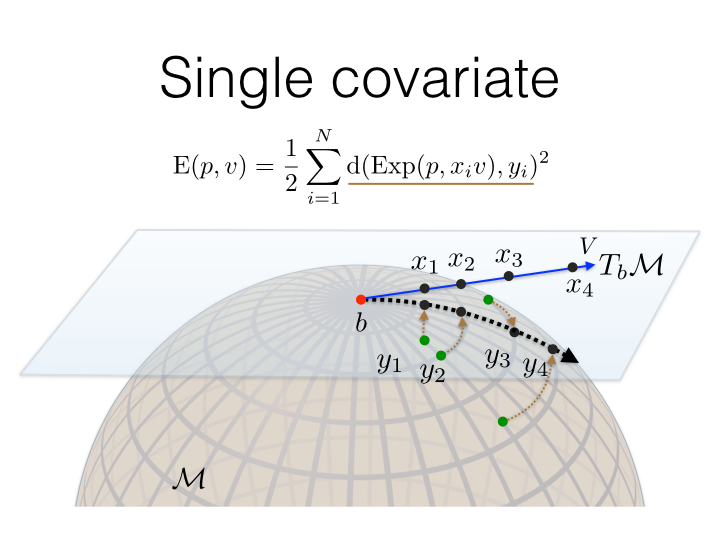
\includegraphics[width=0.49\textwidth,trim={10 40 10 220},clip]{chap2/MGLM2.png}
  \caption{\small\label{fig:manifold}Group-wise MMGLM: The left and right figures represent two linear models on the $\SPD(p)$ manifold. Points $x_i$ in the tangent space are our covariate or predictor, and points $y_i$ in the manifold space represent $\SPD(p)$ matrices. In our regression setting, we wish to minimize the error (brown curves) between the estimation and the sample points. Because each linear model has a different base point, the trajectories cannot be directly compared as in the Euclidean setting.}
\end{figure*}

%Part of the reason is the difficulty of 
This will involve parameterizing {\em trends} in the highly structured nature of the `response' variable ($\SPD$ matrices). 
%In contrast, w
Parametric formulations for manifold-valued data {\em have} been proposed recently \citep{hjkimcvpr2014,cornea2016regression}. %, albeit only in the 
%context of regression models and dictionary learning \citep{xie2013nonlinear}. 
%This result is relevant --- b
Because $\SPD$ matrices form a Riemannian manifold, algorithms
that estimate a parametric model respecting the underlying Riemannian metric are more suitable in many applications as opposed to assuming a Euclidean metric 
on positively or negatively curved spaces \citep{xie2010statistical, fletcher2007riemannian, jayasumanakernel}. We will make a few simple modifications 
(for efficiency purposes) to such algorithms and make use of the estimated parameters for follow-up analysis. 

%Unfortunately, their deployment for the $\SPD$ may not always be trivial.

{\em Finding Group-wise Differences.} Assuming that we have a black-box procedure to estimate a parametric model on the $\SPD$ manifold available, 
in many tasks, such an estimation is merely a segue to other analyses designed to answer scientifically meaningful questions. 
For example, we are often interested in asking whether the temporally coupled model estimated using the procedure above differs 
in meaningful ways {\em across} groups induced by a stratification or dichotomous variable (e.g., gender or disease). For instance, is the `slope' in structured response space statistically different 
across education level or body mass index? 
%in if this model differs significantly across two groups.
While the body of work for graphical model estimation is mature, the literature describing hypothesis tests in this
regime \citep{diffnet,belilovsky2015hypothesis}
is sparse at best.

Given that such questions are simpler to answer with alternative schemes (with assumptions on the distributional properties of the data), e.g., structural equation modeling, 
latent growth models and so on \citep{ullman2003structural, mcardle2000introduction}, it seems that 
the unavailability of such tools is limiting the adoption of such ideas in a broader 
cross-section of science. We will seek to address this gap. 

\begin{figure}[h]
    \centering
    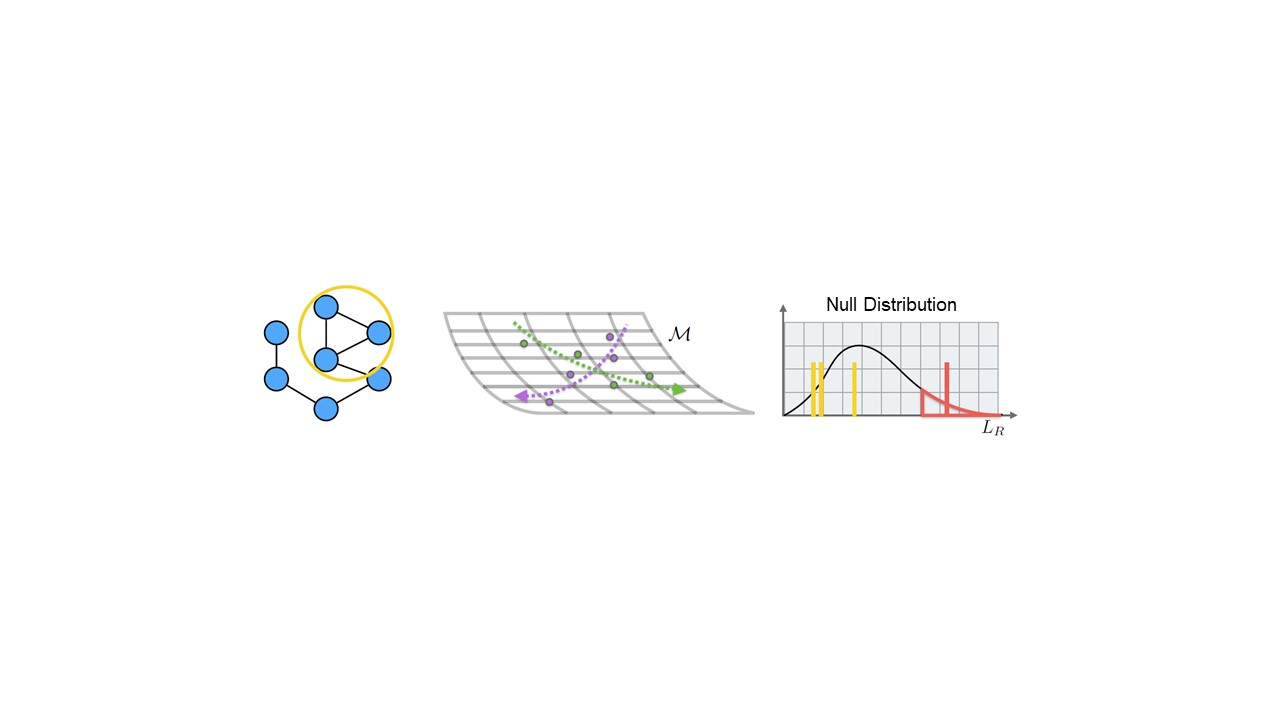
\includegraphics[width=\columnwidth,trim={6.5cm 7.5cm 6.5cm 7.5cm},clip]{chap2/method.jpg}
    \caption{\small\label{fig:model} Our proposed method involves (1) electing a subset of features, (2) fitting manifold regressions on empirical covariances for both groups (green and purple) and (3) constructing the likelihood ratio statistic and comparing it against the null distribution via permutation testing.}
\end{figure}

{\em Needles in Temporal Haystacks.} If we temporarily set aside the potential value of a hypothesis test framework for temporal 
trajectories in graphical models, we see that
from an operational viewpoint, such procedures are most effective when a practitioner already has a precise scientific question in mind. In reality, however, 
many data analysis tools are deployed for exploratory analyses to inform an investigator as to which questions to ask. 
Being able to ``localize'' which parts of the model are different across groups can be very valuable. This ability actually 
benefits statistical power as well. Notice that when the stratified groups are not very different 
to begin with, e.g., healthy individuals with presence or absence of a genetic mutation, the
effect sizes (statistical difference between two groups) are likely to be poor.
Here, while the trends identified on the {\em full} precision matrix may still be different (i.e., there may be a {\em real} signal 
associated with a grouping variable), 
they may not be strong enough to survive significance thresholds. Ideally, what we need here are analogs of the widely used ``scan statistics'' 
for our hypothesis testing formulations for temporal graphical models --- to identify which {\em parts of the signal} are promising. 
Then, even if only a small subset of 
features were different across groups,
%(whereas the complement of this sub-graph were similar, i.e., not different)
we may be able to identify these differential effects efficiently. This benefits Type 2 error, 
provides a practical turnkey product for an experimental scientist, and makes up the key technical results of our work.

Briefly, we provide \textbf{(i)} a simple and efficient parametric procedure for modeling temporally evolving graphical models, \textbf{(ii)} a 
hypothesis test for identifying differences between group-wise estimated models, and \textbf{(iii)} a scan
algorithm to identify {\em those subsets of the features which contribute to the group-wise differences}.
Together, these ideas offer a framework for identifying group-wise differences in temporally coupled graphical models.
%We next cover preliminary concepts, we define our model and present an algorithm, followed by experimental results on both simulated data and neuroimaging data 
%acquired from 
From the experimental perspective, we find scientifically plausible results on 
a unique longitudinally tracked cohort of middle-aged (and young elderly) persons at risk for Alzheimer's disease due to family history, 
but who are otherwise completely cognitively healthy. % COVTRAJ
\chapter{Enabling Temporal Neural Networks via Geometric Tensor Representations} \label{chap:ott} 

While feature selection dates back to classical statistics, 
\textit{parameter selection} has only recently been
studied as
the dimensionality and complexity of models grows
linearly with the size of modern neural networks.
Recurrent Neural networks (RNNs) and its variants are the de facto 
tool of choice 
for modeling sequential data in machine learning and vision.
%For high-dimensional data, a large problem initially faced by these models included exploding/vanishing gradients. 
But until only recently, these models have been severely limited in their ability to model high-dimensional data.
Recurrent structures often lead to large model sizes dependent on sequence length, and thus also require an equivalent number of increased computation.
While RNNs have been successfully applied to video data in some cases, the strategy 
requires problem specific innovations because of the large mapping necessary 
from inputs to hidden representations. It is fair to say that the growth 
in the number of model parameters in various types of 
recurrent models remains a serious bottleneck for high 
dimensional datasets. 
%
% Convolutional neural networks (CNNs), on the other hand, 
% %better suited at 
% handle high dimensional data
% %Modern deep learning architectures now almost exclusively use Convolutional neural networks (CNNs) %to alleviate this issue. 
% %CNNs, partly due to how most networks in broad use today are set up,
% far better and 
% can reduce the dimension of an input significantly by deriving rich feature maps. Most computer vision tasks involve some form of a CNN within the architecture, but incorporating CNNs within recurrent structures 
% seamlessly to mitigate the RNN specific model size issues described above is not always straightforward. Notice that a direct replacement of input and output layers with CNNs leads to a shrinkage of the sequence length considerably \cite{srivastava2015unsupervised}, and pre-training CNN layers may lead to poor local minima when we train without using an end-to-end pipeline \cite{donahue2015long}. Some recent works suggest the use of dilated convolutional networks 
% for sequence modeling \cite{yu2015multi} to partly mitigate these issues, but this line of work is still in its early stages. 
%A similar issue exists with other 
For model-size reduction, both for RNN style networks and otherwise, 
PCA or random projections \cite{ye2005two,bingham2001random} style ``compression" ideas have 
also been used with varying degrees of success.

An interesting perspective on the effective degrees of freedom afforded 
by a given network, a surrogate for the actual ``size'' of the architecture, 
is provided by tensor methods.
% and traces its roots to early 
%results in approximation theory and numerical linear algebra. 
%distinct but related line of work is on t
Tensor decomposition based methods have recently been shown to enable low dimensional representations of very high dimensional data, 
and while these ideas were known to be effective in the ``shallow" regime much earlier, new results also demonstrate their applicability for deep neural 
networks. 
In particular, in the last year, we see a number of tensor based methods being successfully adapted for deep neural network design and compression \cite{cohen2016expressive,zhang2017tucker,yu2017compressing}.
Specifically, \cite{pmlr-v70-yang17e} shows that these compression methods can be very effective in reducing the parameter cost of weight layers in RNNs, enabling simple video analysis tasks that previously would have been computationally prohibitive.

Our goal is to design rich sequential or recurrent models to analyze a longitudinal sequence of high dimensional 3D brain images. 
This task raises two major issues. {\bf First}, 
unless the model size is parsimonious, we find that merely instantiating the 
model with data involving 3D images over multiple time points, even on multiple high end GPU instances, is challenging.
{\bf Second}, 
the eventual goal of medical image analysis is either scientific discovery or generating 
actionable knowledge for patient betterment. 
Both goals require evaluating a model's confidence via 
classical or contemporary statistical techniques: for instance, how confident is the model of its prediction?  
Most, if not all, available tools for assessing 
model uncertainty of deep neural network models 
have a strong dependence on the number of parameters in 
the model. Therefore, even if the first issue above could be mitigated by clever implementation ideas, purely as a practical 
matter, the design of rich and expressive models with a small number of parameters yields immense benefits for calculating model uncertainty.

We tackle the problem of modeling 
sequential 3D brain imaging data using 
recurrent/sequential models. 
Our development starts from well known results on tensor decomposition, and in particular, we
make use of the tensor train representation, which has been shown to be effective in several 
applications in vision and machine learning. We derive a reformulation of the decomposition using 
orthogonality constraints and show that while this makes the estimation slightly more challenging, 
it reduces the number of parameters by as much as half. 
We present a novel parameter estimation scheme based on Stiefel manifold optimization and demonstrate 
how the end to end construction yields benefits for convergence and uncertainty estimation. 
Finally, from the empirical side, we discuss how we enable analysis of and prediction using sequential 3D brain imaging datasets, which to our knowledge is the first such result using 
deep recurrent/sequential architectures. 
 % OTT
\chapter{Efficient Learning and Unlearning via Large-Scale Conditional Independence Testing} \label{chap:lcodec} 

While from one perspective we may be able to constrain our parameter space to one which is desirable,
it may be the case that we cannot
affect or intervene in the model prior to training.
In these cases, 
we may still wish to identify a \textit{subset of existing parameters} that are important or related to particular samples or sample subsets.
As personal data becomes a valuable commodity, legislative efforts have begun to push back on its widespread collection/use particularly for training ML models. Recently, a focus is the ``right to be forgotten" (RTBF), i.e., the right of an individual's data to be deleted from a database (and derived products).
Despite existing legal frameworks on fair use, industry scraping has led to personal images being used without consent, e.g. \cite{Exposing}.
Large datasets are not only stored for descriptive statistics, but used in training large models.
While regulation (GDPR, CCPA) has not specified the extent to which data must be forgotten, it poses a clear question: is  deletion of the data enough, or does a model trained on that data also needs to be updated?

Recent work by \cite{carlini2019secret,carlini2020attack} has identified scenarios where trained models are vulnerable to attacks that can reconstruct input training data. More directly, recent rulings by the Federal Trade Commission \cite{ftc,ftc2} have ordered companies to fully delete and destroy not only data, but also any model trained using those data.
While deletion and (subsequent) full model retraining without the deleted samples is possible, most in-production models require weeks of 
training and review, with extensive computational/human resource cost. With additional deletions, it is infeasible to retrain each time a new delete request comes in. 
% So, are there updates to the model that ensure the data has been deleted (or at least approximately deleted), and full retraining can be postponed?
% Existing works have answered this question in the affirmative, but the computational burden has limited their broad use.
So, how to update a model ensuring the data is deleted without retraining?

{\bf Task.} Given a set of input data $\cS: \{z_i\}_{i=1}^n \sim \mathcal{D}$ of size $n$, training simply identifies a hypothesis $\hat{w} \in \cW$  via an iterative scheme $w_{t+1} = w_t - g(\hat{w},z')$ until convergence, where $g(\cdot,z')$ is  a stochastic gradient of a fixed loss function. Once a model at convergence is found, \textit{machine unlearning} aims to identify an update to $\hat{w}$ through an analogous {\em one-shot unlearning update}:
\begin{align}\label{eq:unlearn}
    w' = \hat{w} + g_{\hat{w}}\left(z'\right),
\end{align}
for a {\em given} sample $z' \in \cS$ that is to be {\bf unlearned}.
%While forms of $g(z')$ have {\color{red}been recently been identified \cite{abc}}, practically they remain infeasible because a complete Hessian computation and inversion is needed. 

\noindent\textbf{Contributions.} We address several computational issues with existing approximate formulations for unlearning by taking advantage of a new statistical scheme for sufficient parameter selection. 
First, in order to ensure that a sample's impact on the model predictions is minimized, we propose a measure for computing conditional independence called L-CODEC which  identifies the Markov Blanket of parameters to be  updated. 
% Extending hypercolumn activations, we identify neural network parameter subsets that are sufficient for model scrubbing.
Second, we show that the L-CODEC identified Markov Blanket enables unlearning in previously infeasible deep models, scaling to networks with hundreds of millions of parameters. 
%{\color{red} with graceful performance degradation}.
Finally, we demonstrate the ability of L-CODEC to unlearn samples and entire classes on networks, from CNNs/ResNets to transformers, including face recognition and person re-identification models. % LCODEC
\chapter{Generalizing the Earth Mover's Distance for Efficient Neural Network Regularization} \label{chap:demd}
Selections of parameters related to individual samples can help with single sample problems,
but the majority of learning problems are more concerned with generalization: if a subset of samples known to be related are behaving differently, can we identify them, and can we remove this difference?
Here, we aim to account for groups of samples that behave differently compared to others, and efficiently regularize models toward fairer solutions.


Optimal transport (OT) has emerged as useful tool for a wide range of applications including information retrieval \cite{balikas2018cross,yurochkin2019hierarchical}, image processing \cite{otip}, statistical machine learning, as well as more recently, for applications in ethics and fairness \cite{kwegyiraggrey2021relative}. 
OT is especially well-suited for tasks where dissimilarity between two or more probability distributions must be quantified,
and its success has been made possible through dramatic improvements in numerical algorithms \cite{cuturi2013sinkhorn,solomon2015convolutional} that allow one to efficiently optimize commonly used functionals.
In practice, OT is often used to estimate and minimize the 
the distance between distributions of interest, 
and this is done using an appropriately defined loss functional. %Recent advances provide us the capability to drop-in and seamlessly integrate many types of losses into existing methods, for novel applications.

%\begin{comment}
%\vikas{the following paragraph is low on content. Perhaps take 1-2 initial lines, compress and use it close off the previous paragraph?}
%The driving practical focus of optimal transport aims to estimate and minimize the distance between distributions of interest. Within machine learning, this takes the form of a loss; recent developments have enabled constructions of such a loss that allow almost seamless integration into existing methods. These incorporations have led to a number of benefits over traditional mean-squared error approaches, taking direct advantage of the statistical and distributional assumptions and requirements of the model fitter.
%\end{comment}

{\bf Barycenters.} 
%{\color{red}Can next two paragraphs merge? Start this with "One way to quantify dissimilarity between many distributions is through distance to the mean....  "} While distances are defined between two points (or two probability distributions), barycenters extend the idea and enable analyzing many points (or probability 
One way to quantify dissimilarity between many distributions is through distance to the mean. Here, for averaging,  
we measure pairwise distances.
Practically, this has led to models that can 
concurrently enforce distributional similarity between a 
set of distributions and has found use in 
a spectrum of applications.

\begin{figure*}[ht]
    \centering
    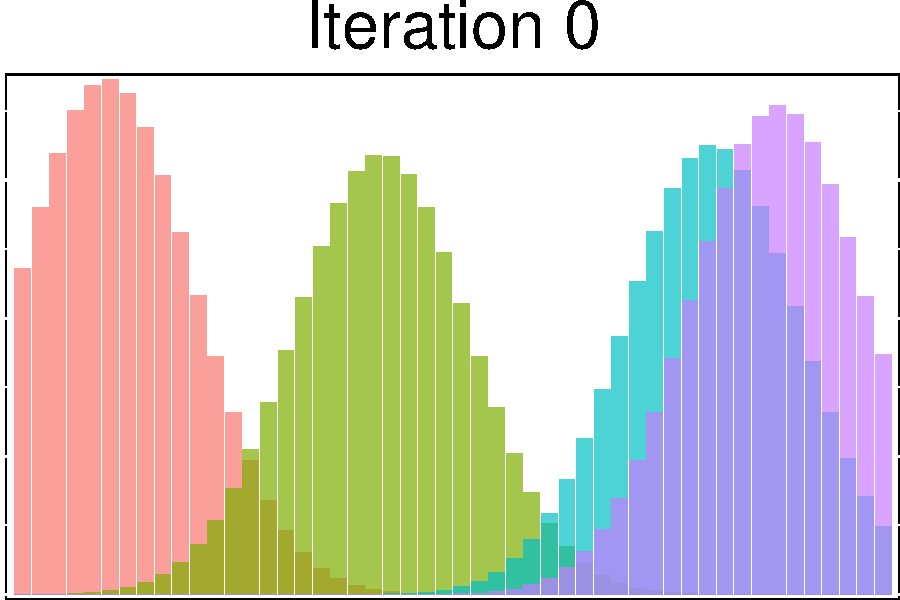
\includegraphics[width=0.19\textwidth]{chap5/hists/hists_iter_0.pdf}
    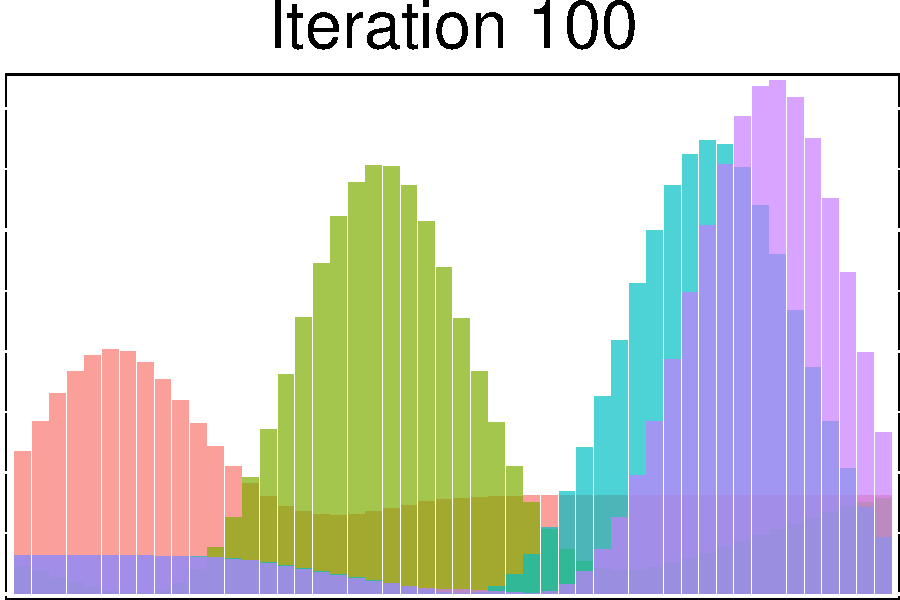
\includegraphics[width=0.19\textwidth]{chap5/hists/hists_iter_100.pdf}
    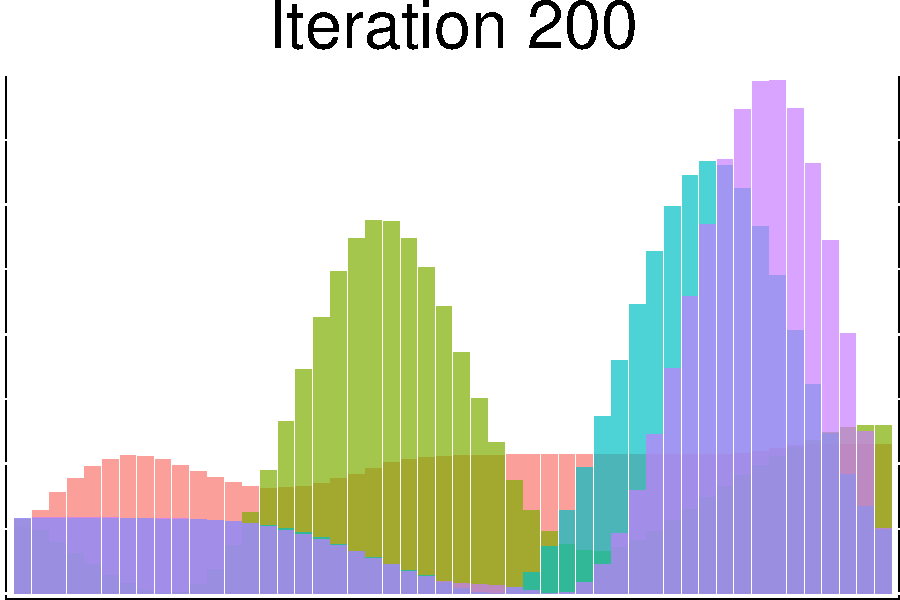
\includegraphics[width=0.19\textwidth]{chap5/hists/hists_iter_200.pdf}
    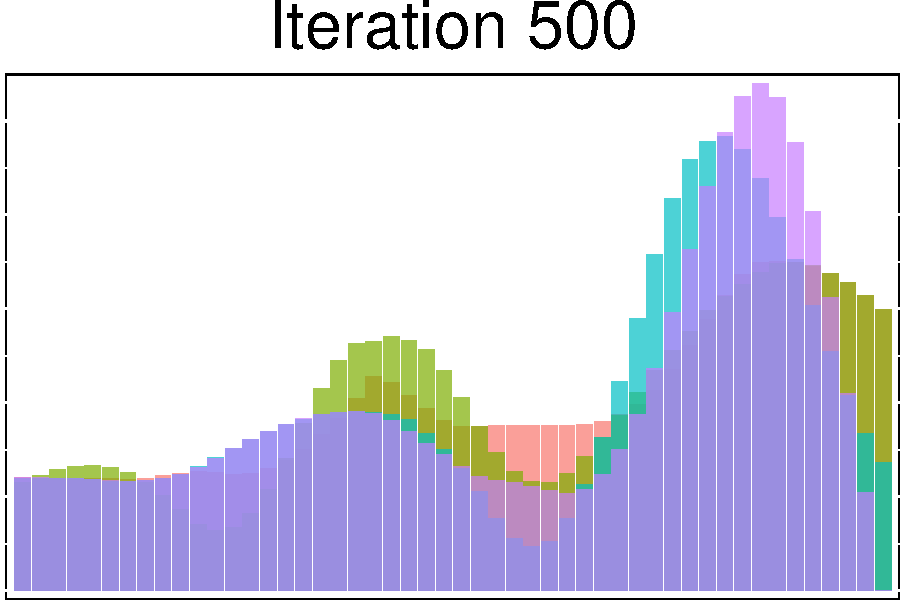
\includegraphics[width=0.19\textwidth]{chap5/hists/hists_iter_500.pdf}
    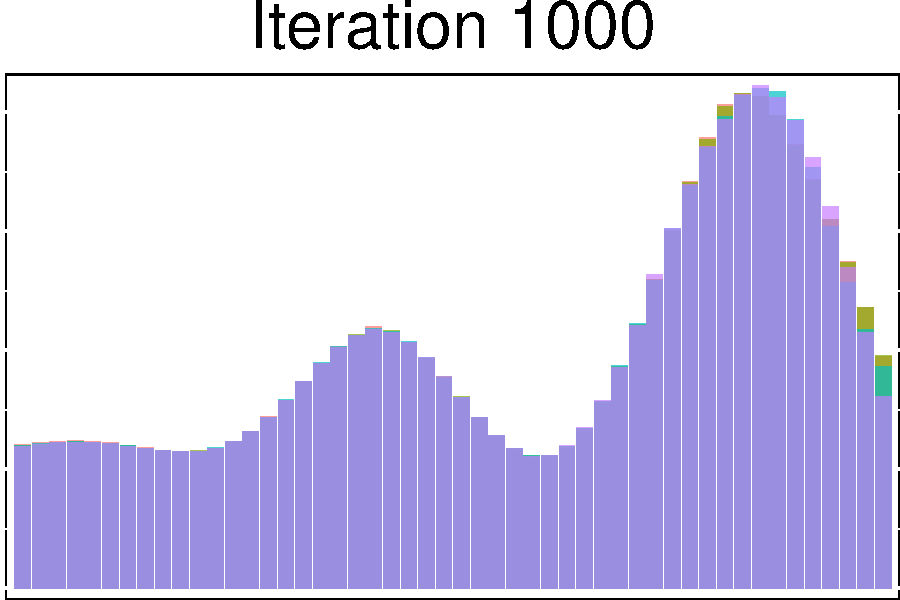
\includegraphics[width=0.19\textwidth]{chap5/hists/hists_iter_1000.pdf}
    \caption{This figure shows the starting and ending state of an iterative process applied to 4 histograms. Each iteration minimizes the generalized Earth Mover's objective, and then updates each histogram in the direction provided by the gradient. Upon each iteration shifts a portion of ``mass'' of every histogram closer to a common distribution. ({\em Left}) The process initially starts with $d=4$ histograms with 50 bins each. ({\em Right}) The update process eventually converges. An intuitive description is that the mass of the original 4 histograms is incrementally shifted around at each step, and all four distributions eventually are reshaped into the limiting distribution, which appears at right. }
    \label{fig:hists}
\end{figure*}

%{\bf Barycenter calculation.} 
Assuming that a suitably regularized form of the optimal transport loss is utilized, the pairwise distance 
calculation is efficient -- in fact, 
in some cases, Sinkhorn iterations can be used \cite{cuturi2013sinkhorn}. 
On the other hand, to minimize distances to the mean, 
most algorithms typically operate 
by repeatedly estimating the barycenter and those pairwise distances, and using a ``coupling'' strategy 
to push points toward the barycenter. 
The idea is sensible but as the number of distributions 
grows, the overall procedure becomes 
computationally intensive.
For example, even on a high end workstation, 
simply computing the barycenter over
50 distributions with 50 bins
%does not converge within a reasonable number of iterations
%using newer packaged solvers. {\color{red} maybe instead of ``not...reasonable'', try ``not competitive"}
proves to be a time-intensive process.
However, very recent research has shown that there exist polynomial time algorithms for this problem 
%have been shown to exist within the last year
\cite{altschuler2021wasserstein}. 
% \vikas{can we concretize it 
% a little more? cite some numbers on a standard workstation? memory requirements? other resource needs?}
 %{\color{red} Glenn: fairness lead}

% {\color{red}this para does not add much}
% Importantly, we should also appreciate that the calculation of the barycenter is often a means to an end in most learning applications -- 
% the ultimate goal tends to be pushing these distributions to come closer. 
% A barycenter is a modeling choice, but other options may also be viable. 
% Indeed, if a different global measure of ``distributional disparity''
% were to be defined and minimized, the costs associated with pairwise comparisons and optimization
% may potentially be avoided. This hypothesis drives much of our development.

\noindent\textbf{Where can we measure dissimilarity?}
% {\color{red} START} Putting aside the cost to compute the barycenter for the moment, 
% instantiations of such applications often desire to enforce distribution similarity
% only on model outputs.
% For example, in \cite{jiang2020wasserstein}, the authors define fairness measures over the probability of the prediction given ground truth labels.  
% This choice is not without good reasons: discrete outputs lead to extremely nice distributions over the probability simplex, where optimization is easy and assumptions need not be strong.{\color{red} END; could START--END be replaced with the gray text?}
In applications, it is often a goal to enforce distribution similarity on model outputs. For example, in \cite{jiang2020wasserstein}, the authors define fairness measures over the probability of the prediction given ground truth labels.   
%FIXME: if you read this and know what X Y and Z are, then fill in and uncomment. This leads to distributions over the probability simplex with the desirable qualities X, Y and Z.
% 
However, these methods are rarely extended to continuous measures within the neural network, 
mainly due to the strong distributional assumptions needed and the added algorithmic complexity of estimating the barycenter.
One drawback of this choice means that the distributional closeness is only guaranteed over the global model output, and little can be said about layer outputs prior to the thresholding for prediction.
Additionally, full retraining would be necessary if thresholds must be adjusted due to changing business or regulatory requirements.

\noindent\textbf{Contributions.} We exploit a recent extension of the classical Earth Movers Distance (EMD) to a higher-dimensional Earth Mover's objective.
We show that minimization of this \textit{global} distributional measure leads to the 
harmonization of input distributions similar in spirit to the minimization of distributions to barycenters.
We prove theoretical properties of the objective and our procedure, and show that 
the gradient can be read directly off from a primal/dual algorithm,
alleviating the need for computationally intense pairwise couplings.
With a particular scaffolding provided by differentiable histograms, we can apply and smoothly operate directly on network activations to compute the EMD measure. 
We establish through experiment that computing gradients used in backpropogation is possible in substantially shorter times than one can achieve using standard tools, due to rapid access to solutions of the the dual linear program formulation.
We compare and contrast the performance and speed of our construction against Barycenter-like measures in a number of settings and demonstrate applications in a common fairness application.
Our final construction integrates seamlessly with existing neural network pipelines, 
which will be publicly available for use.

\begin{figure*}[t]
    \centering
    %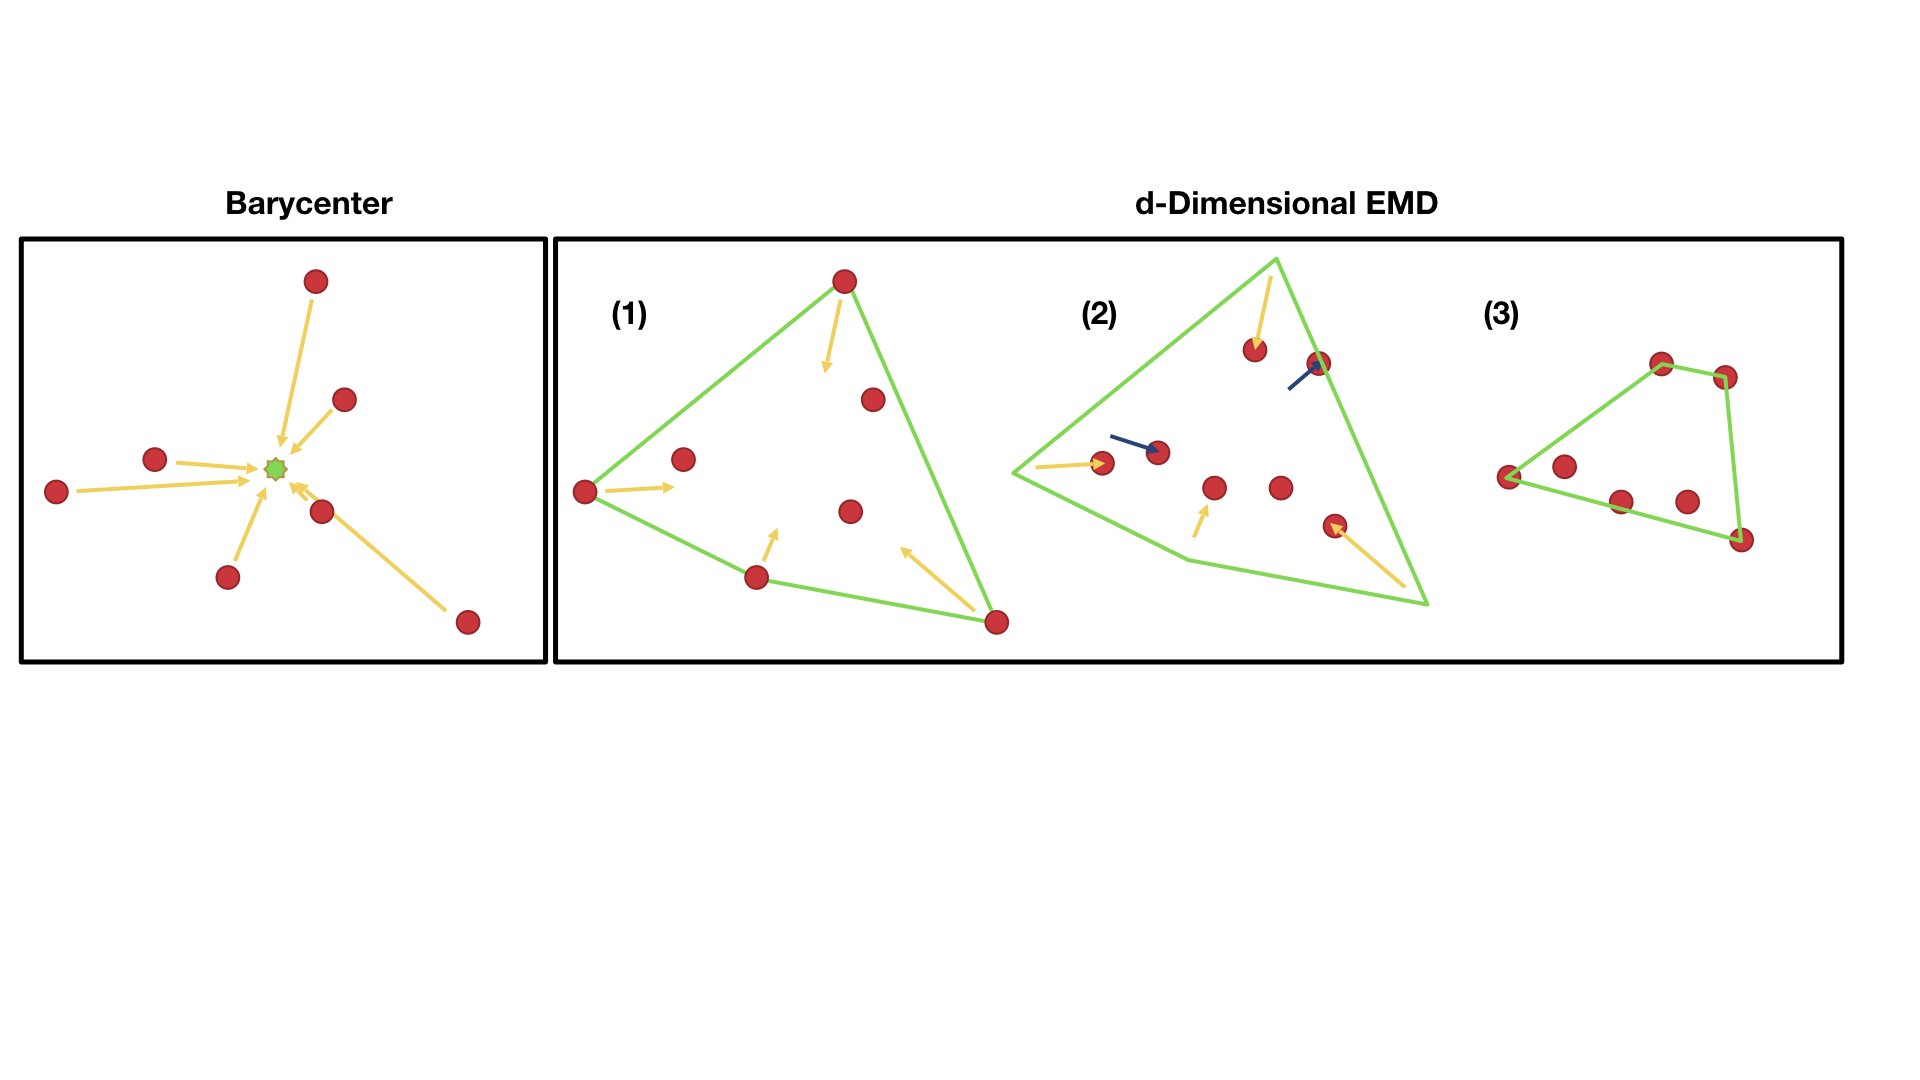
\includegraphics[trim={0 14.5cm 2cm 5cm},clip,width=\textwidth]{figs/demd_abstract.png}
    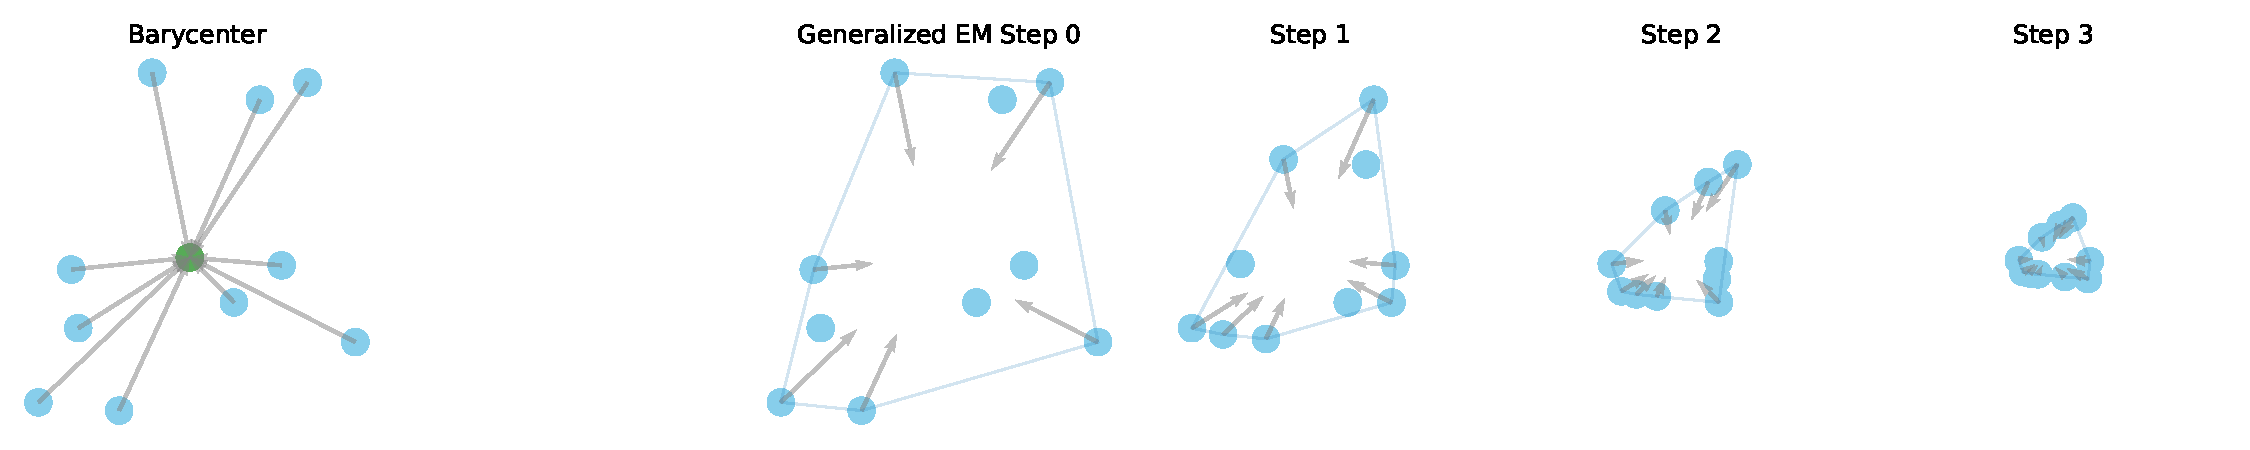
\includegraphics[width=0.95\textwidth]{chap5/bary-gem-step.pdf}
    \caption{({\em Left}) Barycenter approaches identify a center (green) and move samples of interest (blue) toward it along the coupling path (grey). ({\em Right}) Our approach identifies ``support" points that lie within the convex hull,  and only those points are moved in a descent direction. The support points are those that contribute to the objective functional, and it is known (see Theorem 2.2 of~\cite{kline2019properties}) that they are not interior points of the convex hull.}
    \label{fig:min_demd}
\end{figure*}
 % DEMD
\chapter{Future Work: Large Scale Analysis of Multi-Site Preclinical Alzheimer's Disease} \label{chap:pac} 

With the above tools in hand, we aim to move towards applying and deploying both conditional independence schemes and efficient EMD-fairness methods to 
the analysis of a new preclinical cohort of individuals at risk for developing Alzheimer's disease.

\textbf{Data.} Here our data consists of patient information pooled across multiple sites. Demographic measures, neuropsychological test results, genetic indicators, and cerebrospinal fluid (CSF) biomarkers were all collected on individuals from three studies: the Adult Children Study (ACS), the Wisconsin Registry for Alzheimer's Prevention (WRAP), and the Biomarkers of Cognitive Decline Among Normal Individuals (BIOCARD). Data was preprocessed using standard pipelines, collated, and harmonized across sites. Table~\ref{tab:pacfeats} details the full list of measures.

\begin{table}[]
    \centering
    \begin{tabular}{l|l}
        \hline\hline
         A$\beta$42 & A$\beta$40 \\
         T-Tau & P-Tau \\
         A$\beta$42/A$\beta$40 & PTAU-A$\beta$42 \\
         Age & Gender \\
         Executive Function & General Cognitive Performance \\
         Episodic Memory & Time \\
         Education & APOE \\
         \hline\hline
    \end{tabular}
    \caption{Preclinical AD Measures used in conditional independence analysis.}
    \label{tab:pacfeats}
\end{table}

Imaging data is also available for a subset of the individuals included in the above set, and future work includes incorporation of these imaging modalities (MRI, DTI, and PET region of interest measures).

\textbf{Methods.} The results shown here demonstrate the potential value of applying conditional independence methods over standard correlation methods. 

\begin{figure}
    \centering
    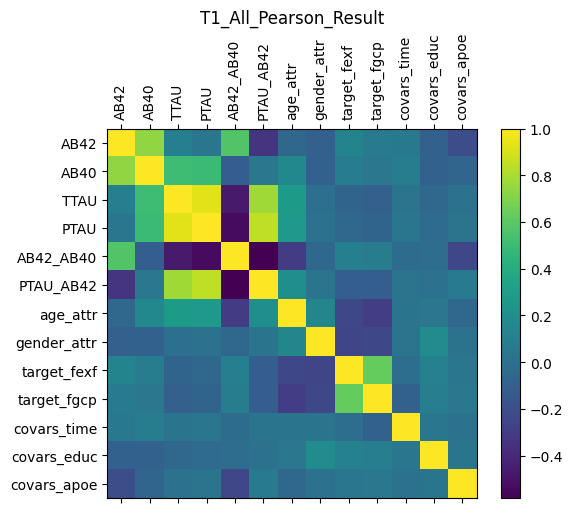
\includegraphics[width=0.24\textwidth]{chap6/figs/T1_All_Pearson_Result.png}
    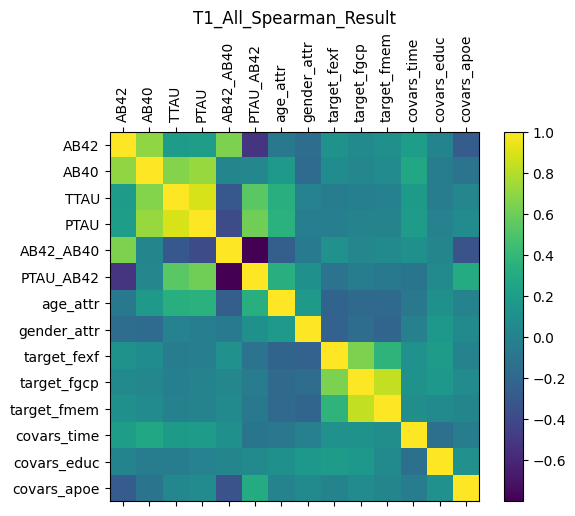
\includegraphics[width=0.24\textwidth]{chap6/figs/T1_All_Spearman_Result.png}
    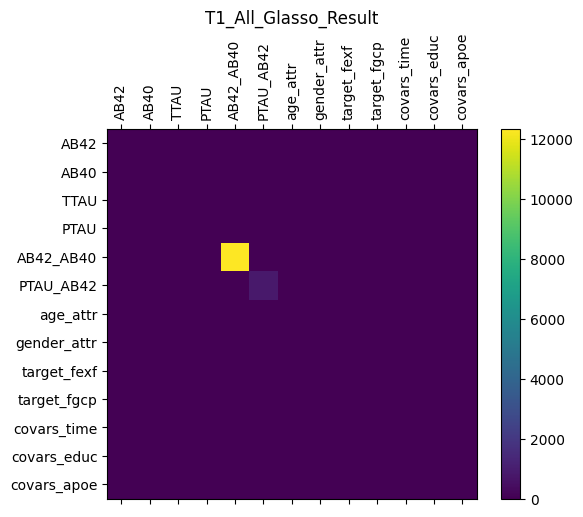
\includegraphics[width=0.24\textwidth]{chap6/figs/T1_All_Glasso_Result.png}
    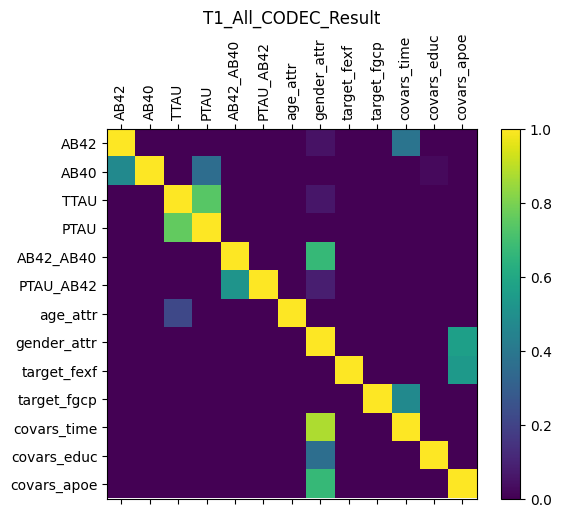
\includegraphics[width=0.24\textwidth]{chap6/figs/T1_All_CODEC_Result.png}
    
    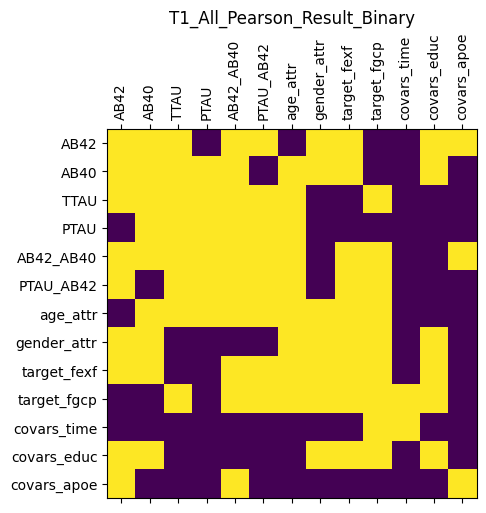
\includegraphics[width=0.24\textwidth]{chap6/figs/T1_All_Pearson_Result_Binary.png}
    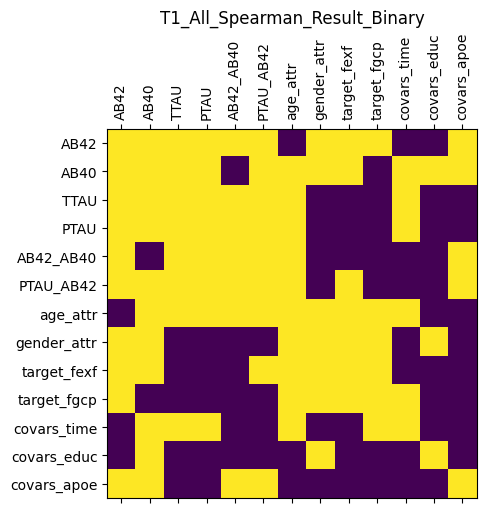
\includegraphics[width=0.24\textwidth]{chap6/figs/T1_All_Spearman_Result_Binary.png}
    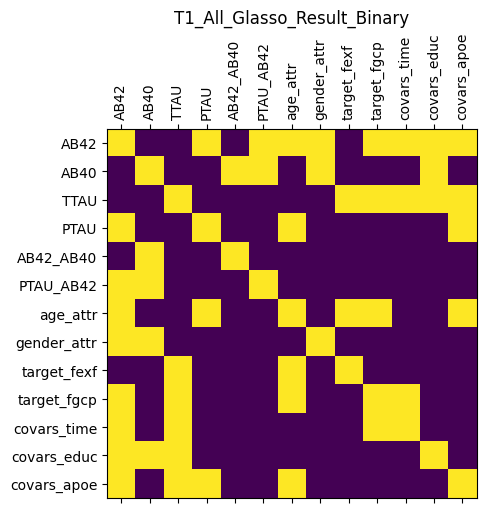
\includegraphics[width=0.24\textwidth]{chap6/figs/T1_All_Glasso_Result_Binary.png}
    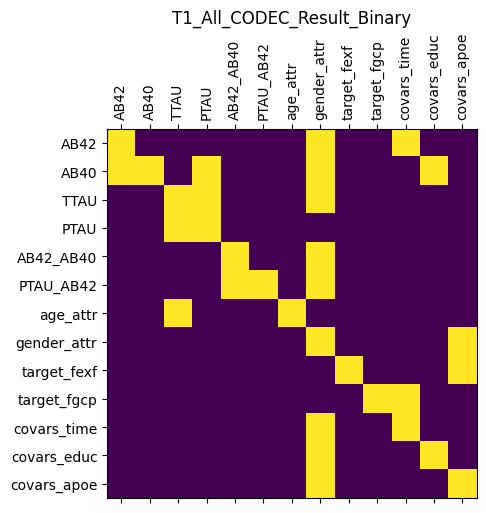
\includegraphics[width=0.24\textwidth]{chap6/figs/T1_All_CODEC_Result_Binary.png}
    \caption{All Sites.}
    \label{fig:all}
\end{figure}

\begin{figure}
    \centering
    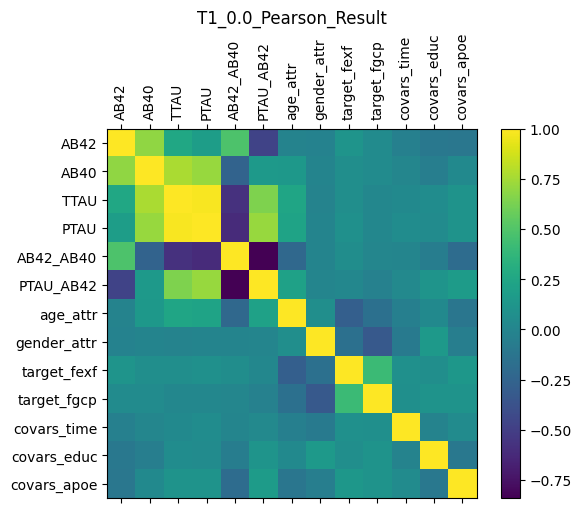
\includegraphics[width=0.24\textwidth]{chap6/figs/T1_0.0_Pearson_Result.png}
    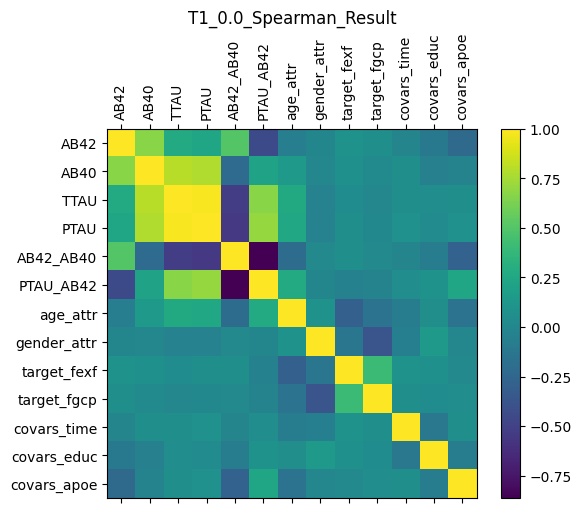
\includegraphics[width=0.24\textwidth]{chap6/figs/T1_0.0_Spearman_Result.png}
    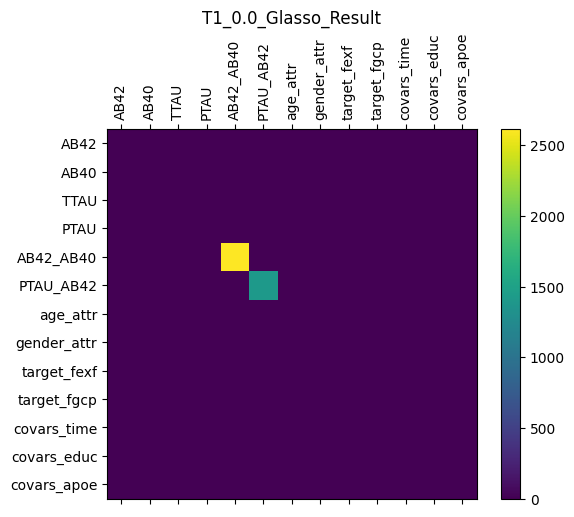
\includegraphics[width=0.24\textwidth]{chap6/figs/T1_0.0_Glasso_Result.png}
    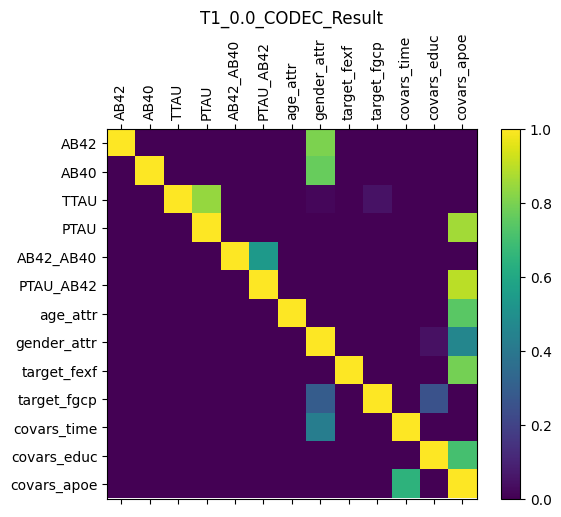
\includegraphics[width=0.24\textwidth]{chap6/figs/T1_0.0_CODEC_Result.png}
    
    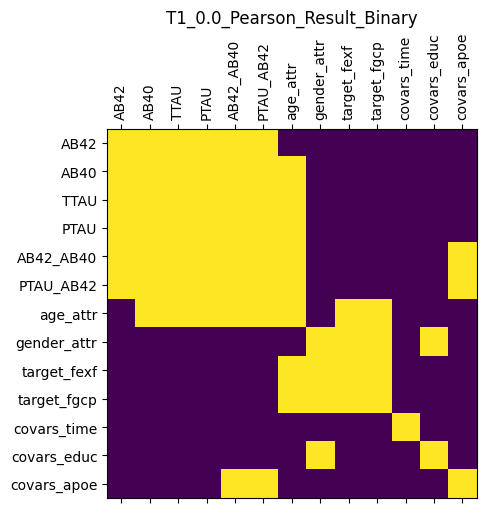
\includegraphics[width=0.24\textwidth]{chap6/figs/T1_0.0_Pearson_Result_Binary.png}
    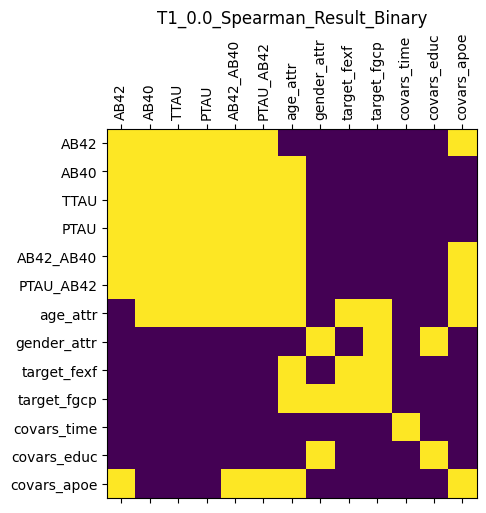
\includegraphics[width=0.24\textwidth]{chap6/figs/T1_0.0_Spearman_Result_Binary.png}
    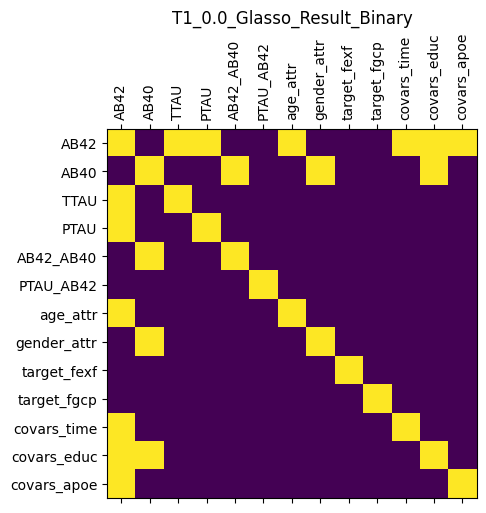
\includegraphics[width=0.24\textwidth]{chap6/figs/T1_0.0_Glasso_Result_Binary.png}
    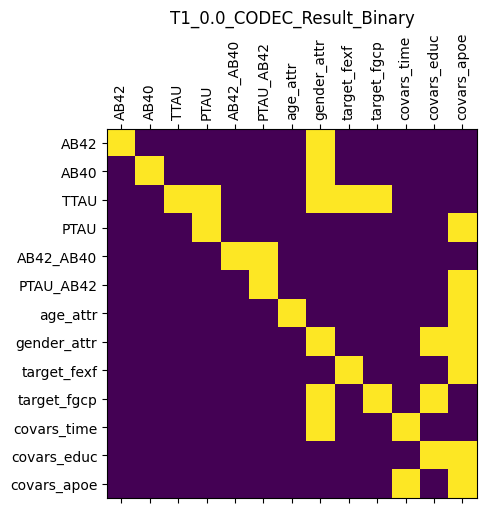
\includegraphics[width=0.24\textwidth]{chap6/figs/T1_0.0_CODEC_Result_Binary.png}
    \caption{Site 0: WRAP.}
    \label{fig:site0}
\end{figure}

\begin{figure}
    \centering
    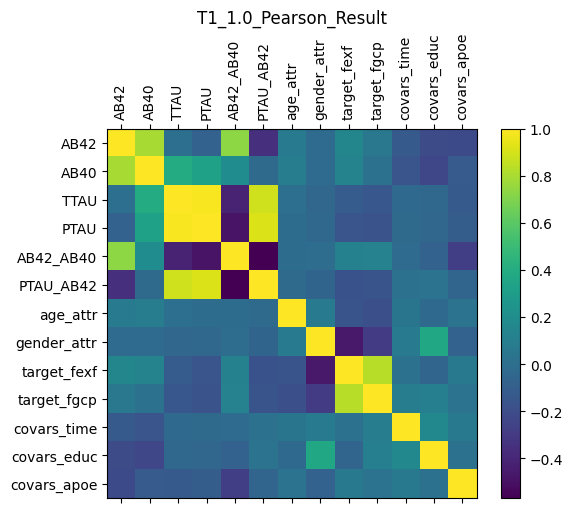
\includegraphics[width=0.24\textwidth]{chap6/figs/T1_1.0_Pearson_Result.png}
    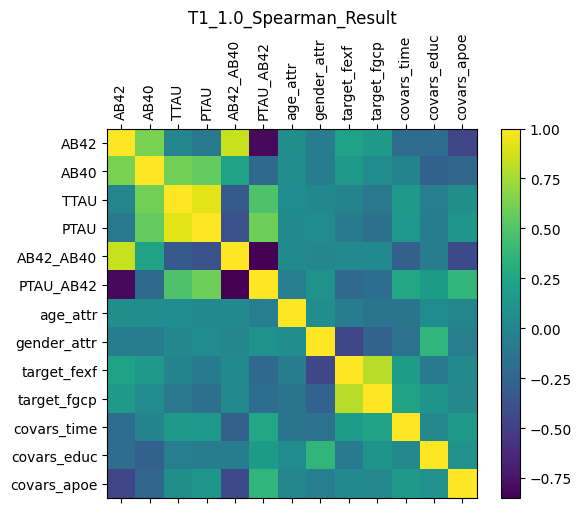
\includegraphics[width=0.24\textwidth]{chap6/figs/T1_1.0_Spearman_Result.png}
    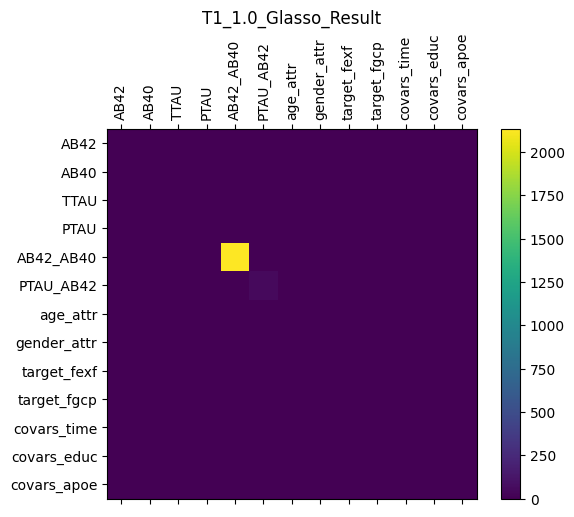
\includegraphics[width=0.24\textwidth]{chap6/figs/T1_1.0_Glasso_Result.png}
    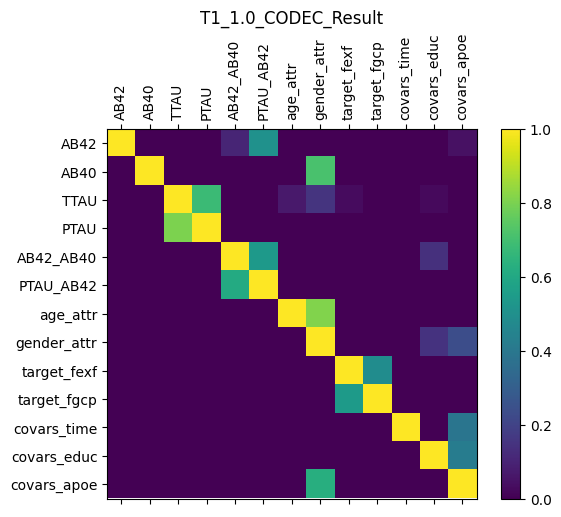
\includegraphics[width=0.24\textwidth]{chap6/figs/T1_1.0_CODEC_Result.png}
    
    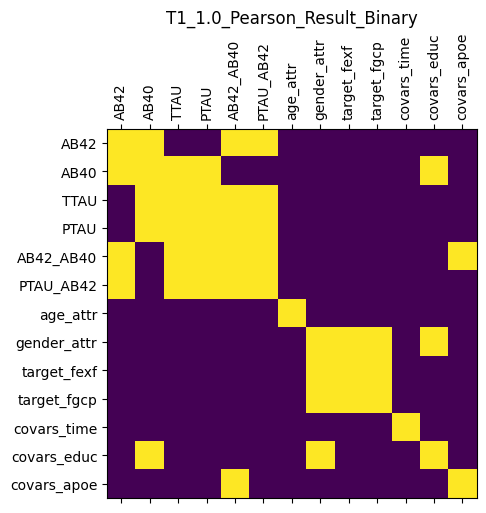
\includegraphics[width=0.24\textwidth]{chap6/figs/T1_1.0_Pearson_Result_Binary.png}
    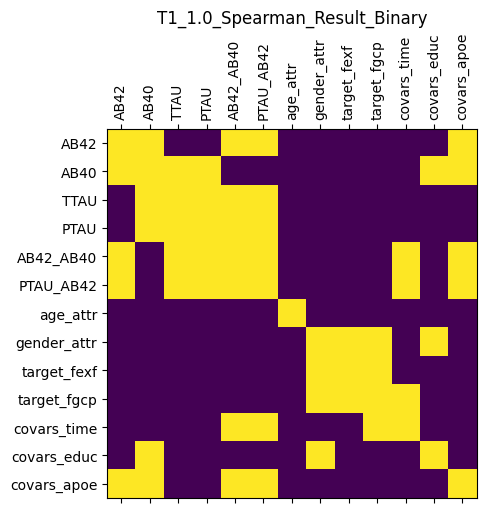
\includegraphics[width=0.24\textwidth]{chap6/figs/T1_1.0_Spearman_Result_Binary.png}
    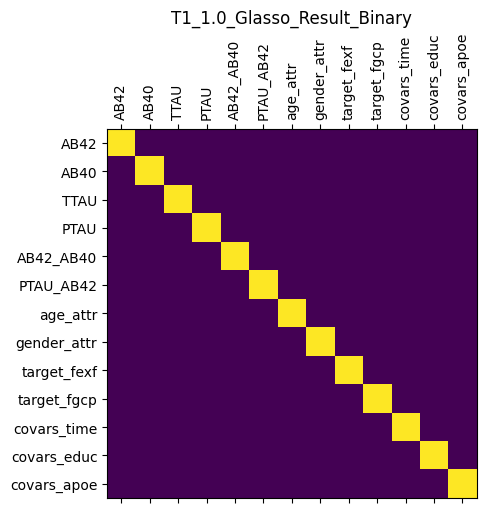
\includegraphics[width=0.24\textwidth]{chap6/figs/T1_1.0_Glasso_Result_Binary.png}
    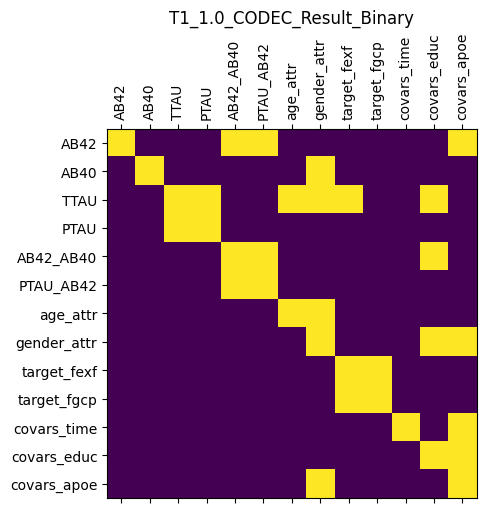
\includegraphics[width=0.24\textwidth]{chap6/figs/T1_1.0_CODEC_Result_Binary.png}
    \caption{Site 1: ACS.}
    \label{fig:site1}
\end{figure}

\begin{figure}
    \centering
    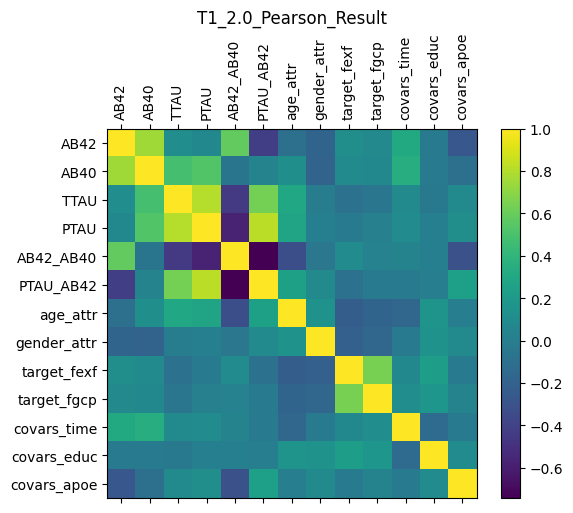
\includegraphics[width=0.24\textwidth]{chap6/figs/T1_2.0_Pearson_Result.png}
    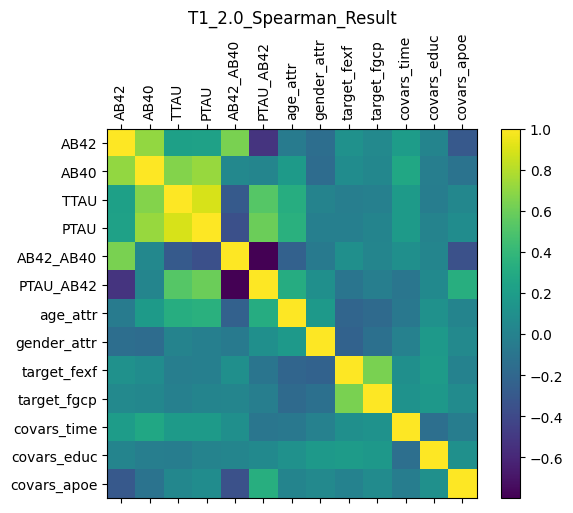
\includegraphics[width=0.24\textwidth]{chap6/figs/T1_2.0_Spearman_Result.png}
    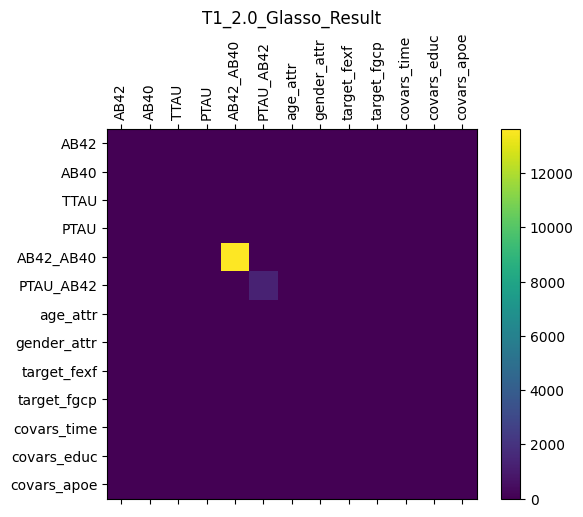
\includegraphics[width=0.24\textwidth]{chap6/figs/T1_2.0_Glasso_Result.png}
    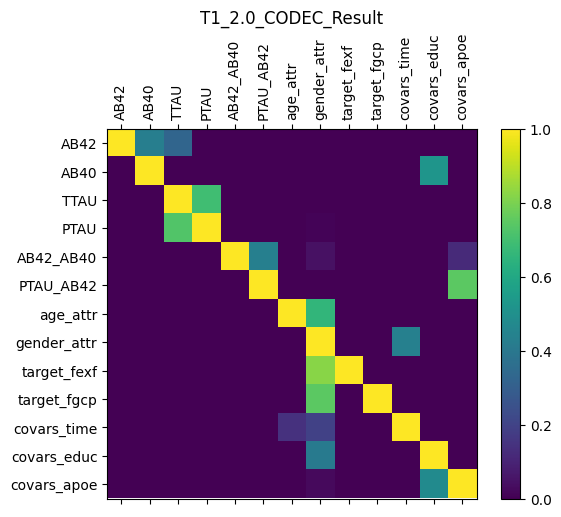
\includegraphics[width=0.24\textwidth]{chap6/figs/T1_2.0_CODEC_Result.png}
    
    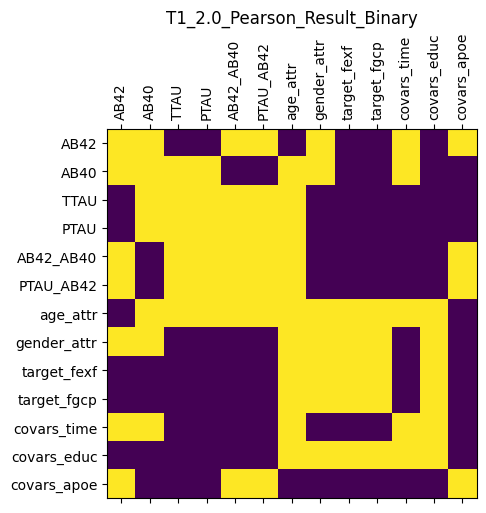
\includegraphics[width=0.24\textwidth]{chap6/figs/T1_2.0_Pearson_Result_Binary.png}
    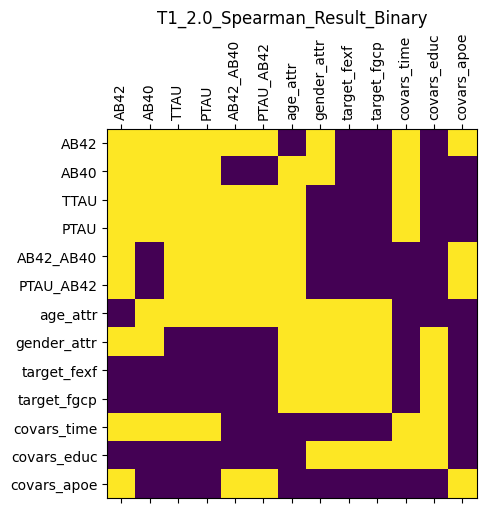
\includegraphics[width=0.24\textwidth]{chap6/figs/T1_2.0_Spearman_Result_Binary.png}
    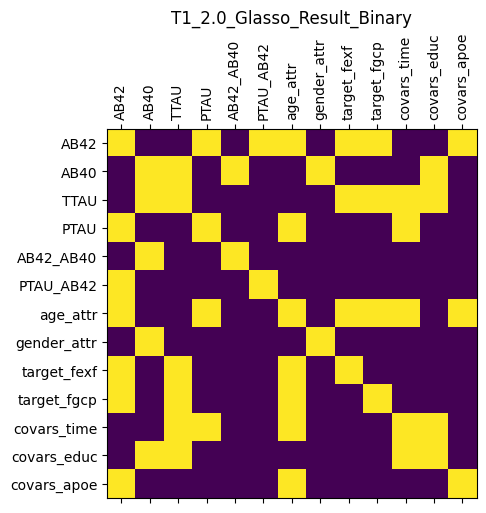
\includegraphics[width=0.24\textwidth]{chap6/figs/T1_2.0_Glasso_Result_Binary.png}
    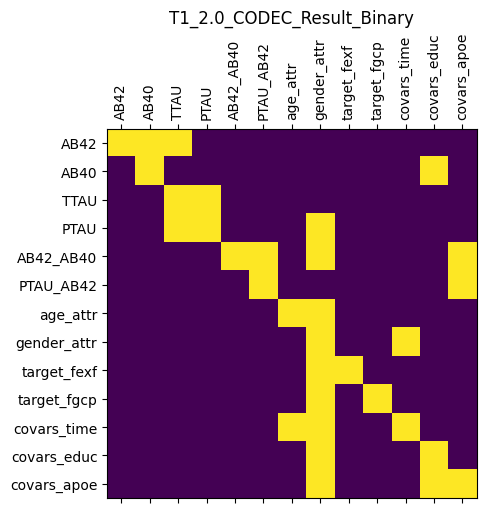
\includegraphics[width=0.24\textwidth]{chap6/figs/T1_2.0_CODEC_Result_Binary.png}
    \caption{Site 2: BIOCARD.}
    \label{fig:site2}
\end{figure} % future-ish
% \chapter{Future work}
lfkajsdlf jaewofj woeig ewoigaweioghaewlih aewlig hewi hwaeoihawioha;oig awe' dfasdf sdaf weg a4 g4w herah t



%% Do you have appendices?  If so, add them here, just like chapters.
% \begin{appendices}
% \include{backmatter/appendix1}
% \end{appendices}


%% McBride is a very nice style (some version is included in this distribution)
\bibliographystyle{mcbride}
% put all you .bib files in bib directory
\bibliography{bib/intro_ref.bib, bib/chap2_ref.bib, bib/chap3_ref.bib, bib/chap4_ref.bib, bib/chap5_ref.bib, bib/chap6_ref.bib}

\end{document}
